\chapter[Spectropolarimetry and the SALT/RSS]{Spectropolarimetry and the \gls{SALT}/\gls{RSS}} \label{ch:02}

This chapter gives an overview of the basics of spectropolarimetry (\autoref{sec:spectropolarimetry}), and how it functions, following from the principles of both spectroscopy (\autoref{sec:spectroscopy}) and polarimetry (\autoref{sec:polarimetry}).
Further, it is discussed how these techniques are practically implemented for \gls{SALT} (\autoref{sec:SALT}), using the \gls{RSS} (\autoref{subsubsec:RSS}), and how the spectropolarimetric reduction process is completed (\autoref{sec:RSS_reductions}).

\section{Spectroscopy} \label{sec:spectroscopy}

Spectroscopy originated in its most basic form with Newton's examinations of sunlight through a prism \citep{opticks} but came to prominence as a field of scientific study with Wollaston's improvements to the optics elements \citep{WollPrism}, Fraunhofer's use of a diffraction grating instead of a prism \citep{FraunGrating}, and Bunsen and Kirchoff's classifications of spectral features to their respective chemical elements \citep{KirBunSpec}.

\begin{figure}[t]
    \centering
    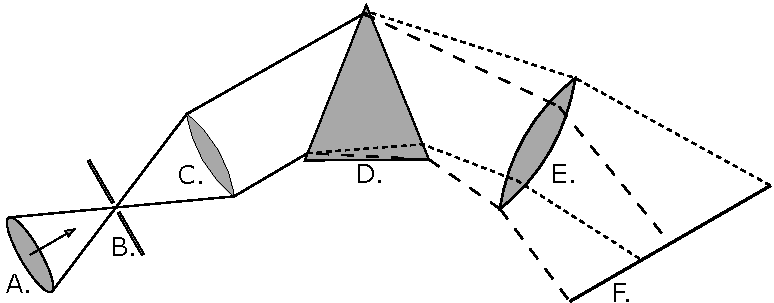
\includegraphics[width = 1.0\textwidth]{2_spectrometer.pdf}
    \caption{
        Layout depicting the light path through a spectrometer.
        Diagram adapted from \cite{BirneyObsAstro}.
    }
    \label{fig:spectrometer}
\end{figure}

% How it works
The simplest spectrometer schematic, as shown in \autoref{fig:spectrometer}, consists of incident light collected from the telescope's optics, labelled A, being focused onto a slit, B, and passed through a collimator, C.
The collimator collimates the light allowing a dispersion element, D, to disperse the light into its constituent wavelengths.
The resultant spectrum is focused by camera optics, E, onto a focal plane, F.
Viewing optics are situated at the focal plane in the case of a spectroscope and a detector is situated at the focal plane in the case of a spectrograph.

\subsection{Telescope Optics}

The telescope optics refers simply to all the components of a telescope necessary to acquire a focal point at the spectrometer entrance, labelled B.
The focal point in most traditional telescope designs is fixed relative to the telescope and so the spectrometer may be mounted at that point.
In cases where the telescope is designed to have a moving focal point relative to the telescope \cite[see][]{Arecibo, HET, SALT_design}, the spectrometer, or a signal transfer method such as a fibre feed to the spectrometer, must also move along the telescope's focal path.

\subsection{Slit}

The slit's function is to control the amount of incident light entering a spectrometer and, along with the exposure time of the detector, prevents over-exposures of bright sources on highly sensitive detectors \citep{TonkPracAmSpec}.
If a source is spatially resolvable, or larger than the seeing conditions, the slit additionally acts to spatially limit the source to increase the spectral resolution, resulting in sharper features in the resultant spectrum.
Without the slit the spectral resolution would be determined by the projected width of the source on the detector, or the seeing if the source was a star-like point source.
Increasing the spectral resolution comes with the trade-off of decreasing the light collected from the source and thus acquiring a less intense resultant spectrum.
Multiple spectra may be acquired simultaneously when the slit is positioned such that collinear sources lie along the slit.

The spectrometer is usually situated at the focal point.
In cases where this is not feasible due to restrictions, for example restrictions of weight or size, a fibre feed may be situated behind the slit on the telescope.
Alternatively, the individual fibres may be rearranged to cover only the slit, altogether removing the need for a slit.
This allows the signal to be routed away from the telescope to a controlled environment with only miniscule losses.

%Spectroscopy done with no slit is commonly referred to as objective spectroscopy and, as the name suggests, the prism is situated just before the telescopes objective, the primary element of the telescope that focuses the collected light to the primary focus.

\subsection{Collimator}

The collimators function is to collimate the focused light from the telescope, ensuring that all light rays run parallel before reaching the dispersion element, as most dispersers are designed to operate in a parallel beam.
The focal ratio of the collimator ($f_{c} / D_{c}$, where $f$ refers to the focal length and $D$ refers to the diameter) should ideally match the focal ratio of the telescope ($f_{T} / D_{T}$).

% Other considerations are also necessary when dealing with collimators, such as the sizing, weight, and price, but which may be of interest but which fall outside of the scope of the basic working principles discussion are unrelated to is ensuring that the full collecting area is utilized as an oversized collimator may be heavier as well as more expensive than necessary.

% as seen in \autoref{eq:focal_ratio}
% \begin{equation}
%     \frac{f}{D} = \frac{f_{1}}{d_{1}}
%     \label{eq:focal_ratio}
% \end{equation}

% From basic trigonometry and a small angle approximation, $\sin(\theta) \approx \theta$, \autoref{eq:small_angle} can be derived.
% From it, it can be seen that as the linear size, $D$, of most stellar objects is much smaller than the distance to those objects, $d$, and thus the incident light is already almost entirely collimated.

% \begin{equation}
% 	\theta (\arcsec) = 206265 \frac{D}{d}
% 	\label{eq:small_angle}
% \end{equation}

\subsection{Dispersion Element}

Including a dispersion element in the optical path is what defines a spectrometer.
As the name suggests, a dispersion element disperses the light incident on it into its constituent wavelengths and produces a spectrum.
There are two types of dispersion elements, namely the prism and the diffraction grating, which operate on different principles, as discussed in \autoref{subsec:dispersion}.

\subsection{Camera Optics}

The lens functions similarly to that of the telescope's optics but in this case focuses the dispersed light onto a receiver situated at the focal plane.
As mentioned previously, an eye piece is fixed to the focal point for a spectroscope while a spectrograph employs a detector.

\subsection{Detector}

The two most prevalent detector types in spectroscopy are the \gls{CCD} and \gls{CMOS} detectors.
In astronomical spectroscopy however, sources are fainter and exposure times are much longer and so the \gls{CCD} detectors are by far the preferred detector as their output has a higher-quality and lower-noise when compared to \gls{CMOS} cameras under the same conditions \citep{CCDvsCMOS}.

The \gls{CCD} is a detector composed of many thousands of pixels which can store a charge so long as a voltage is maintained across the pixels.
Each pixel detects incoming photons using photo-sensitive capacitors through the photoelectric effect and converts the photons to a charge \citep{CCDastronomy}.
There are also thermal agitation effects which introduce noise to the charge accumulated by a pixel, further discussed in \autoref{subsec:calibration}.
Once the exposure is finished the accumulated charge is read column by column, row by row, through an Analog-to-Digital Converter which produces a two-dimensional array of `counts'.

% Each \gls{CCD} image may be referred to by a name such as a bias, dark, flat field, or science image, which helps the observer differentiate the purpose of each image, also further discussed in \autoref{subsec:calibration}.

\subsection{Dispersion of Light} \label{subsec:dispersion}

Light can be broken up into its constituent wavelengths through two different physical phenomena, namely dispersion and diffraction, which dispersive elements use to create spectra.
Dispersive prisms and diffractive gratings each have their strengths and weaknesses and a wide spectrum of instruments exist which implement either, or both, concepts.
Regardless of the specific element, dispersive elements all have a resolving power, $R$, and an angular dispersion.
Generally, while the angular dispersion is a more involved process to determine, the resolving power of a spectrograph can be measured as:
\begin{equation} \label{eq:resolving_power}
    R = \frac{\lambda}{FWHM}\,,
\end{equation}
where $\lambda$ is the wavelength of an incident monochromatic beam and \gls{FWHM} refers to the width of the spectral line on the detector at half of its maximum intensity.

\subsubsection{Prism} \label{subsubsec:prism}

\begin{figure}[t]
    \centering
    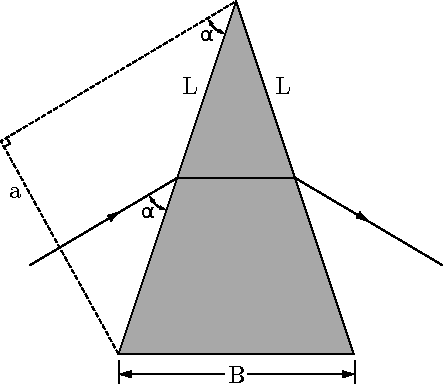
\includegraphics[width = 1.0\textwidth]{2_prism_diagram.pdf}
    \caption{
        Geometry of a prism refracting an incident monochromatic beam at a minimum deviation angle.
        Diagram adapted from \cite{BirneyObsAstro}.
    }
    \label{fig:prism_diagram}
\end{figure}

The prism operates on the principle that the refractive index of light, $n$, varies as a function of its wavelength, $\lambda$.
Prisms were the only dispersive elements available for early spectroscopic studies, but they were not without flaw.
The angular dispersion of a prism is given by:
\begin{equation} \label{eq:prism_angular_dispersion}
    \frac{\partial \theta}{\partial \lambda} = \frac{B}{a}\frac{dn}{d\lambda}\,,
    % \propto -\lambda^{-3}
\end{equation}
where $\theta$ is the angle at which the refracted light differs from the incident light, $\lambda$ is the wavelength of the incident light, $B$ is the longest distance the beam would travel through the prism.
$a = L \sin(\alpha)$ is the maximal beam width that would fit onto a prism with a transmissive surface of length $L$ for a given angle, $\alpha$, at which a beam would strike the transmissive surface, as shown in \autoref{fig:prism_diagram}.

The refractive index of a material as a function of its wavelength, $n(\lambda)$, can be approximated by Cauchy's equation:
\begin{equation} \label{eq:Cauchy}
    n(\lambda) = A_{C} + \frac{B_{C}}{\lambda^{2}} + \frac{C_{C}}{\lambda^{4}} + \dots\,,
\end{equation}
where $A_{C}$, $B_{C}$, and $C_{C}$, etc., are the Cauchy coefficients and have known values for certain materials.
Cauchy's equation is a much simpler approximation of the refractive index that remains very accurate at visible wavelengths \citep{JenkinsOptics}.
Taking only the first term of the derivative of the Cauchy equation allows us to approximate the angular dispersion of a prism,
\begin{equation} \label{eq:prism_angular_dispersion_approx}
    \begin{aligned}
        \frac{\partial \theta}{\partial \lambda} &= -\frac{B}{a}\frac{2B_{C}}{\lambda^{3}} \\
        \therefore\; \frac{\partial \theta}{\partial \lambda} &\propto -\frac{1}{\lambda^{3}}\,,
    \end{aligned}
\end{equation}
which shows that the angular dispersion of a prism is wavelength dependent and furthermore that longer wavelengths are dispersed less than shorter wavelengths \citep{BirneyObsAstro, Hecht_optics}.
The dependence of the angular dispersion, $d\theta/d\lambda$, on the wavelength, $\lambda$, is crucial for the formation of spectra but this cubic, non-linear, relation results in a non-linear spectrum.
Since prisms rely on the refractive index of the material they are made of, they have low angular dispersions.

Multiple prisms can be used to increase the angular dispersion but as the dispersion is non-linear it becomes increasingly more difficult to calibrate.
The more material and material boundaries the light must pass through, the more its intensity decreases due to attenuation effects and Fresnel losses.
Even so, the transmittance of modern prisms for their selected wavelength range is generally very high due to improved manufacturing methods as well as improved transmitting materials.\footnote{See manufacturers technical specifications, \href{https://www.thorlabs.com/newgrouppage9.cfm?objectgroup_id=148}{THORLABS}, or \href{https://www.edmundoptics.eu/c/prisms/607/}{Edmund Optics} for example.}

\subsubsection{Diffraction Grating} \label{subsubsec:diff_grat}

\begin{figure}[t]
    \centering
    
\includegraphics[width = 1.0\textwidth]{2_grating_diagram.pdf}
    \caption{
        Geometry of a reflective blazed grating refracting an incident monochromatic beam.
        Diagram adapted from \cite{BirneyObsAstro}.
    }
    \label{fig:grating_diagram}
\end{figure}

The alternative dispersing element is a diffraction grating, which operates on the principle that as light interacts with a grating where the groove size is comparable to the light's wavelength, the light is dispersed through constructive and destructive interference.
This interference results in multiple diffracted beams $m$, called orders, either side of a central reflected, or transmitted, beam such that $m \in Z$, where $m = 0$ is the non-dispersed, or reflected, beam.

An example of a reflective blazed grating is illustrated in \autoref{fig:grating_diagram}.
Here a monochromatic beam is incident on the grating at an angle of $\alpha$ from the grating normal.
Due to the interference, a diffracted beam of wavelength $\lambda$ is found at an angle of $\beta$ from the grating normal.
The relation between the incident and diffracted beams is given by the grating equation:
\begin{equation} \label{eq:grating_equation}
    m\lambda = \sigma (\sin(\alpha) \pm \sin(\beta))\,,
\end{equation}
where $\sigma$ is the groove spacing of the grating and $m$ is the order of the diffracted beam being considered.
The grating equation also applies to transmission gratings, though care should be taken for the signs of $\alpha$ and $\beta$.

% It is important to note that the sign of $\alpha$ and $\beta$ depend on whether the grating is reflective or transmissive.
% In the case of a reflective grating, such as in \autoref{fig:grating_diagram}, the signs of $\alpha$ and $\beta$ are the same relative to the grating normal, $\lambda = \sigma (\sin(\alpha) + \sin(\beta))$ for $m = 1$.
% In the case of a transmissive grating, the signs of $\alpha$ and $\beta$ are the opposite relative to the grating normal, $\lambda = \sigma (\sin(\alpha) - \sin(\beta))$ for $m = 1$.

% Free Spectral range and Blazing
\autoref{eq:grating_equation} also shows that different diffracted beams may share an angle of dispersion for beams not in the same order.
The regions of an order that do not overlap with another order are called free spectral ranges.
An order-blocking filter may be used to account for the overlaps and increase the free spectral range.
A diffraction grating can also be blazed by an angle $\theta$, as illustrated in \autoref{fig:grating_diagram}.
Blazing refers to the fact that the grooves on the surface of the grating are not symmetrical.
The asymmetry of the grooves diffracts the incident beam such that most of the beam's intensity is found in a reflected ($\beta = \alpha$) $0^{th}$ order beam.
The wavelength at which a blazed spectrograph is most effective is called the blaze wavelength, $\lambda_{b}$, which is determined by:
\begin{equation} \label{eq:blaze_wavelength}
    \begin{aligned}
        m\lambda_{b} &= 2\sigma\sin(\theta)\cos(\alpha - \theta)\rlap{\,,\ where}\\
        2\theta &= \alpha + \beta\,.
    \end{aligned}
\end{equation}

% Angular dispersion
Taking the derivative of \autoref{eq:grating_equation} with respect to $\lambda$ while keeping $\alpha$ constant, allows us to determine the angular dispersion of a diffraction grating,
\begin{equation} \label{eq:grating_angular_dispersion}
    \frac{\partial \beta}{\partial \lambda} = \frac{m}{\sigma \cos(\beta)}\,.
\end{equation}
It is important to realize that the values for $m$ and $\sigma$ are not chosen independent of other parameters, and thus the ratio $m / \sigma$ may be substituted with the grating equation, resulting in
\begin{equation} \label{eq:grating_angular_dispersion_subbed}
    \begin{aligned}
        \frac{\partial \beta}{\partial \lambda} &= \frac{1}{\lambda} \frac{\sin(\alpha) + \sin(\beta)}{\cos(\beta)}\,.
    \end{aligned}
\end{equation}
\autoref{eq:grating_angular_dispersion_subbed} may be seen as a combination of two terms, a wavelength dependent term and an `angular' term which is dependent on the grating geometries.
For realistic grating configurations at optical wavelengths the angular dependence varies quite slowly as compared to the wavelength dependence, and so the spectral dispersion may be approximated as:
\begin{equation} \label{eq:grating_angular_dispersion_approx}
    \frac{\partial \beta}{\partial \lambda} \propto \frac{1}{\lambda}\,.
\end{equation}

Similar to the dispersion of a prism, \autoref{eq:grating_angular_dispersion_approx} shows that the dispersion of a grating is predominantly wavelength dependent, but this dependence is only inversely proportional and thus more uniform across a wavelength range than that of a prism.
Furthermore, shorter wavelengths are refracted less than longer wavelengths since there is no negative relation between the angular dispersion and the wavelength \citep{BirneyObsAstro, Hecht_optics,MKS_Handbook}.

\subsubsection{Alternate Diffraction Elements}

As mentioned before, multiple subgroups exist for both dispersive prisms and diffractive gratings.
For prisms, along with the single and multiple prism setups mentioned, there also exists grisms and immersed gratings.
A grism (Grating Prism), as shown in \autoref{fig:grism}, refers to a transmissive grating etched onto one of the transmissive faces of a prism and allows a single camera to capture both spectroscopic and photometric images without needing to be moved, with and without the grism in the path of the beam of light, respectively.
An immersed grating refers to a grism modified such that the transmissive grating is coated with reflective material.
The primary source of dispersion for both grisms and immersive gratings is the grating and any aberration effects from the prism are negligible in comparison.

\enlargethispage{-1\baselineskip}

\begin{figure}[t]
    \centering
    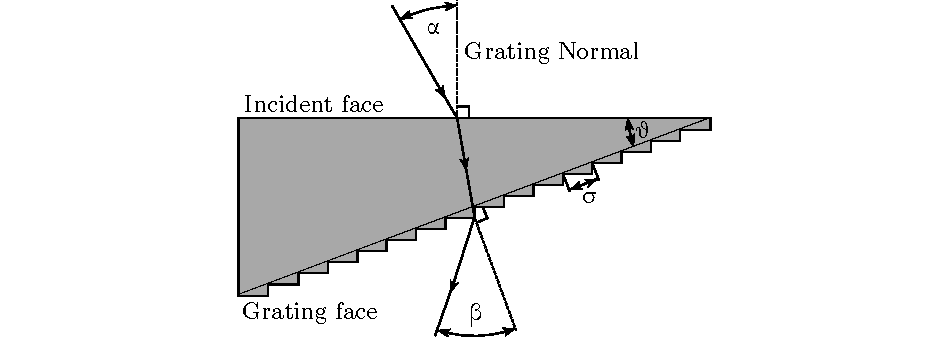
\includegraphics[width = 1.0\textwidth]{2_grism.pdf}
    \caption{
        Diagram of a grism for an incident monochromatic beam of light and a diffracted beam of order $m = 1$.
        Diagram adapted from \cite{BirneyObsAstro}.
    }
    \label{fig:grism}
\end{figure}

% Echelle and VPH grating
Other types of gratings include the \gls{VPH} grating as well as the echelle grating.
The \gls{VPH} grating consists of a photoresist, which is a light-sensitive material, sandwiched between two glass substrates.
Diffraction is possible since the photoresist's refractive index varies near-sinusoidally perpendicularly to the gratings lines, as seen in \autoref{fig:vph_grating}.
This allows for sharper diffraction orders and low stray light scattering as compared to more traditional gratings but since blazing is not possible the efficiency is decreased.
An echelle grating refers to a diffraction grating with higher groove spacing which is optimized for use at high orders.
The high order of the diffracted beam allows for greater angular dispersion which is most useful when combined with another dispersion element to cross-disperse a spectrum, resulting in a high resolution spectrum.

\begin{figure}[t]
    \centering
    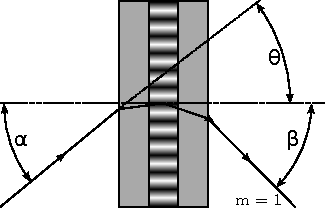
\includegraphics[width = 1.0\textwidth]{2_vph_grating.pdf}
    \caption{
        Diagram of a \gls{VPH} grating for an incident monochromatic beam of light.
        Diagram adapted from \cite{BirneyObsAstro}.
    }
    \label{fig:vph_grating}
\end{figure}

\subsection{Detector and Spectroscopic Calibrations} \label{subsec:calibration}

Acquiring a spectrum from observations is more involved than simply reading out the data recorded on the \gls{CCD}.
A raw science image, which is the raw counts of the observed source read from the \gls{CCD} with no calibrations applied, has on it a combination of useful science data as well as noise.
The noise is a combination of random noise introduced through statistical processes and systematic noise introduced through the instrumentation and the observation conditions the source was observed under.
This noise causes an uncertainty in the useful data and can be minimized, predominantly by calibrating for the systematic noise, but never fully removed \citep{CCDhandbook}.

The dominant source of noise in a raw image is detector noise.
\glspl{CCD} are manufactured to have a small base charge in each pixel, called the `bias' current which allows the readout noise, a type of random noise, to better be sampled.
There is also an unintentional additional charge which is linearly proportional to the exposure time and originates from thermal agitation of the \gls{CCD} material, called the `dark' current.
The dark current can be minimized and possibly ignored if the \gls{CCD} is adequately cooled.
These types of noise add to the charge held by a pixel and are thus considered additive.

\pagebreak

\begin{figure}[t]
    \centering
    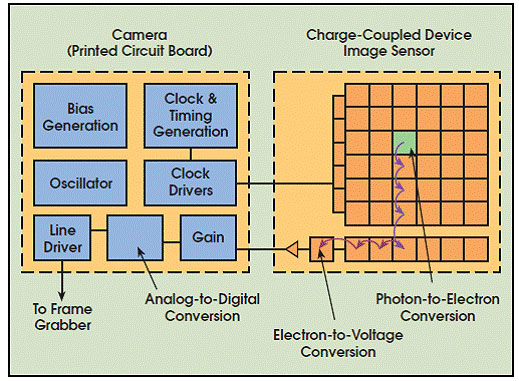
\includegraphics[width = 10cm]{2_ccd.jpg}
    \caption{
        Diagram of the inner logic of a \gls{CCD}.
        Figure adapted from \cite{ccd_fig}.
    }
    \label{fig:ccd_diagram}
\end{figure}

The \gls{CCD} is not a perfect detector and the efficiency of it and the optics of the telescope also contribute noise to the image.
The efficiency of a \gls{CCD} is referred to as the Quantum Efficiency, and it is a measure of what percentage of light striking the detector is actually recorded and converted to a charge.
The efficiency of the \gls{CCD} and telescope optics is also wavelength dependent and so the noise that results from them is more complex than that of additive noise.
This type of noise is referred to as multiplicative noise.

Additive noise, such as bias and dark currents, is inherent to \gls{CCD} images, and as such needs to be subtracted out first when performing calibrations.
Bias currents can be found by taking a bias image or by adding an overscan region to each image.
A bias image is an image where the charges on the \gls{CCD} are reset and then immediately read off without exposing anything on the detector, effectively taking an image with zero exposure time.
Alternatively, to save time during an observational run, overscan regions may be added to the images.
An overscan region refers to adding a few cycles to the readout of each column of the \gls{CCD} such that the base current is read out and appended to each image.

Dark currents can be found by taking an image with nothing exposed onto the detector for a certain exposure time.
This resultant dark image can then be scaled to the science images exposure time since the dark current should be linearly proportional to exposure time.
When the detector is capable of being held at precise temperatures, dark images may be taken over multiple hours during the day to produce a high quality master dark image that may then be scaled and subtracted from all subsequent images, after bias subtractions.

Next, multiplicative noise, such as a \gls{CCD}s pixel-to-pixel response, should be accounted for.
This pixel-to-pixel response should be uniform across the image and to achieve this an average response may be divided out.
The average response is referred to as a `flat' image or flat-field and may be acquired by observing a uniformly illuminated surface to determine the pixel-to-pixel response.

\pagebreak

Dome flats are images taken of a relatively flat surface, usually the inside of a telescopes dome, and are used in both photometry and spectroscopy.
The surface is uniformly and indirectly illuminated by a projector lamp, ideal for flat-field images.
Alternate flat-fielding methods, such as night sky and twilight flats, are available but are more suited for photometry than spectroscopy.
Twilight flats may be used for spectroscopy when the instrumental response over the length of the slit must be calibrated for, when observing extended objects for example.

Night sky flats are produced from science images containing mostly sky.
The science images are combined using the `mode' statistic which removes any celestial objects at the cost of a low \gls{SNR} flat-field.

Twilight flats are produced from images of the twilight (or dawn) sky.
They are taken when the Sun has just set, in the opposite direction, at $\sim 20$\degree\ from zenith and provide a better \gls{SNR} at the cost of careful timing of the images.

A flat-field must be normalized before being used to correct any science images since it only acts to account for the pixel-to-pixel response and not for the additive errors.
A  normalized spectroscopic flat image, $F^{n}_{\lambda}(x,y)$, can be calculated as:
\begin{equation} \label{eq:norm_flat}
    F^{n}_{\lambda}(x,y) = \frac{F_{\lambda}(x,y) - B(x,y) - (\frac{t_{S}}{t_{D}})D(x,y)}{\text{med}_{lp}(F_{\lambda}(x,y) - B(x,y) - (\frac{t_{S}}{t_{D}})D(x,y))}\,,
\end{equation}
where $F_{\lambda}(x,y)$ is the non-corrected flat image, $B(x,y)$ is the bias image, $D(x,y)$ is the dark image which is scaled by the exposure time of the science image, $t_{S}$, and the dark image, $t_{D}$.
med$_{lp}$ is a low-pass median filter which smoothes out any rapid changes in the pixel-to-pixel response, removing the illumination contribution.

The calibrated science image, $S^{*}_{\lambda}(x,y)$, which accounts for the bias and dark currents as well as the flat fielding can then be calculated as:
\begin{equation} \label{eq:science_cal}
    S^{*}_{\lambda}(x,y) = \frac{S_{\lambda}(x,y) - B(x,y) - (\frac{t_{S}}{t_{D}})D(x,y)}{F^{n}_{\lambda}(x,y)}\,.
\end{equation}

When multichannel \glspl{CCD} are used, which consist of multiple \glspl{CCD} or a \gls{CCD} with multiple output amplifiers, additional calibrations, specifically cross-talk corrections and mosaicking, are required.
Cross-talk noise refers to contamination that occurs during readout in one channel from another channel with a high signal and occurs because the signals can not be completely isolated from one another.
Cross-talk corrections therefore account for this signal contamination between channels being read out at the same time \citep{CrossTalk}.

Mosaicking is necessary for multichannel \glspl{CCD} since the digitized signal read out from the detector has no reference of the physical location of the pixel it was detected at.
Mosaicking, therefore, correctly orients the data acquired from a multichannel detector so that a single correctly oriented image is produced.

\begin{figure}[t]
    \centering
    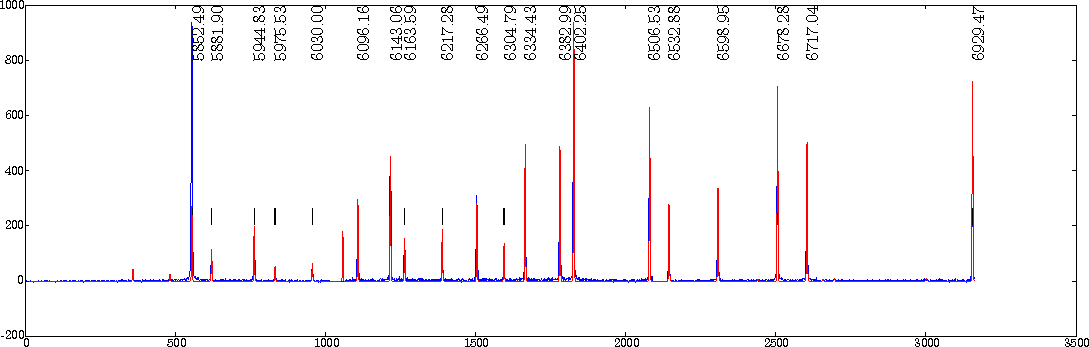
\includegraphics[width = 16cm]{2_Ne_arc.pdf}
    \caption{
        Example of an arc spectrum for NeAr taken with the \gls{SALT}/\gls{RSS} using the PG1800 grating at a grating angle of $34.625$\degree, an articulation angle of $69.258$\degree, and covering a wavelength range of $\sim 5600$ -- $6900$~\AA.
        Plot adapted from the \gls{SALT} published Longslit Line Atlases, (2023).\protect\footnotemark
    }
    \label{fig:Ne_arc}
\end{figure}
\footnotetext{\protect\href{http://pysalt.salt.ac.za/lineatlas/plot_line_neon.pdf}{NeAr plot} sourced from \protect\url{https://astronomers.salt.ac.za/data/salt-longslit-line-atlas/}}

\subsubsection{Wavelength Calibration}

Finally, since the dispersion element breaks the incident light into its constituent wavelengths non-linearly (\autoref{subsec:dispersion}), the relation between the pixel on a detector and the wavelength of the light incident on it is unknown.
Ideally, the spectrometer's optics would be modeled to produce a reliable pixel to wavelength calibration \citep[see e.g.,][]{WavCalSpectraModel}, but this becomes increasingly more difficult for spectrometers with complex, non-sedentary, optical paths.

Alternatively, a source with well-defined spectral features, with said features evenly populating the wavelength region of interest, such as in \autoref{fig:Ne_arc} may be observed.
The observed frame is commonly referred to as an `arc' frame, after the arc-lamps used to acquire the spectra, and should be observed alongside the science frames over the course of an observation run.

It is important that the arc frame is observed at the same observing conditions and parameters as the science frames since the optical path will vary over the course of an observing run and for different observing parameters, invalidating previously acquired arc frames.
The wavelength calibrations then consist of defining a two-dimensional pixel-to-wave\-length conversion function from the arc frame which may later be applied to calibrate the science frames.
The two most common approximations for wavelength calibrations are the Chebyshev and Legendre polynomial approximations.

\begin{figure}[t]
    \centering
    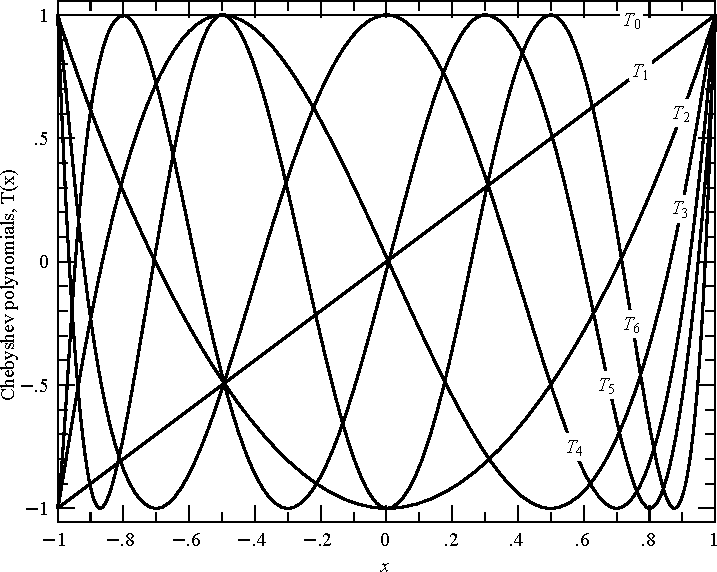
\includegraphics[width = 12cm]{2_chebyshev.pdf}
    \caption{
        The first seven Chebyshev polynomials ($T_0$ through $T_{6}$) as defined by \autoref{eq:chebypoly} over the region $[-1, 1]$ for which they are orthogonal.
        Plot adapted from \citep{numerical_recipes}.\protect\footnotemark
    }
    \label{fig:chebyshev}
\end{figure}
\footnotetext{Excellent resources on Chebyshev and Legendre polynomials are available digitally at \protect\href{http://numerical.recipes/book}{www.numerical.recipes/book}.}

\paragraph{Chebyshev Polynomials}

The Chebyshev polynomials are defined explicitly as:
\begin{align} \label{eq:chebypolyexplicit}
    T_{n}(x) &= \cos(n \cos^{-1}(x))\,,
\end{align}
or recursively as:
\begin{align}
    T_{0}(x) &= 1 \,,\notag\\
    T_{1}(x) &= x \rlap{\,,\ and} \label{eq:chebypoly}\\
    T_{n+1}(x) &= 2xT_n(x) - T_{n-1}(x) \rlap{\,,\ for $n \geq 1$\,,}\notag
\end{align}
where $T$ is a Chebyshev polynomial of order $n$.%
\footnote{Chebyshev polynomials are denoted $T$ as a hold-over from the alternate spelling of `Tchebycheff'.}
An important property of Chebyshev polynomials is that they are orthogonal polynomials.
This means that the inner product of any two differing Chebyshev polynomials, $T_{i}(x)$ and $T_{j}(x)$, over the range $[-1, 1]$ is zero, as shown by:
\begin{equation} \label{eq:chebyorth}
    \int_{-1}^{1} T_{i}(x) T_{j}(x) \frac{1}{\sqrt{1-x^{2}}} \,dx =
    \begin{cases}
        0,       & i \neq j     \\
        \pi / 2, & i = j \neq 0 \\
        \pi,     & i = j = 0
    \end{cases}\,,
\end{equation}
where $1 / \sqrt{1 - x^{2}}$ is the weighting factor for Chebyshev polynomials.
This property is important because it means that the coefficients in the Chebyshev polynomial expansion are independent of one another, allowing for a unique solution when approximating an unknown function \citep{numerical_recipes, cheby}.
A Chebyshev approximation of an unknown wavelength calibration function is given by:
\begin{align} \label{eq:chebyshev}
    f(x) &\approx \sum_{i = 0}^{N}  c_{i} T_{i}(u)\rlap{\,,\ or}\\
    F(x, y) &\approx \sum_{i = 0}^{N} \sum_{j = 0}^{M} c_{ij} T_{i}(u) T_{j}(v)\,,\label{eq:chebyshev2D}
\end{align}
for a one- or a two-dimensional wavelength surface function, respectively.
Here $N$ and $M$ are the desired $x$ and $y$ orders, and $c_{i}$ and $c_{ij}$ are the Chebyshev polynomial coefficients \citep{chebysurf, cheby2d}.
Since the orthogonality property of the Chebyshev polynomials only holds true over the range $[-1, 1]$, the $(x, y) \in ([0, a], [0, b])$ pixel coordinates must be remapped to $u, v \in [-1, 1]$ following the relation:
\begin{equation} \label{eq:XtoUV}
    (u, v) = \frac{2 (x, y) - a - b}{b - a}\,.
    % (x, y) &= \frac{b - a}{2} (u, v) + \frac{a+b}{2}
\end{equation}
The Chebyshev polynomials are more suited for wavelength calibrations than standard polynomials since they are orthogonal and have minima and maxima located at $[-1, 1]$, as seen in \autoref{fig:chebyshev}.
This means that the Chebyshev approximation is exact when $x = x_{n}$, where $x_{n}$ are the positions of the $n - 1$ $x$-intercepts of $T_{N}(x)$.
These properties greatly minimize the error in the Chebyshev approximation, even at lower orders \citep{cheby}.

% When the calibration function is known but the function cannot be evaluated, the coefficients, $c_{n}$, may be approximated by:
% \begin{equation}
%     c_{n} \approx \frac{2}{N} \sum_{k = 0}^{N - 1} f(x_{k}) T_{n}(x_{k})\,,\label{eq:chebycoeff}
% \end{equation}

% \begin{equation}
%     x_{n} = \cos{\left(  \frac{\pi}{2} \frac{2 n + 1}{N} \right)}
% \end{equation}

\begin{figure}[t]
    \centering
    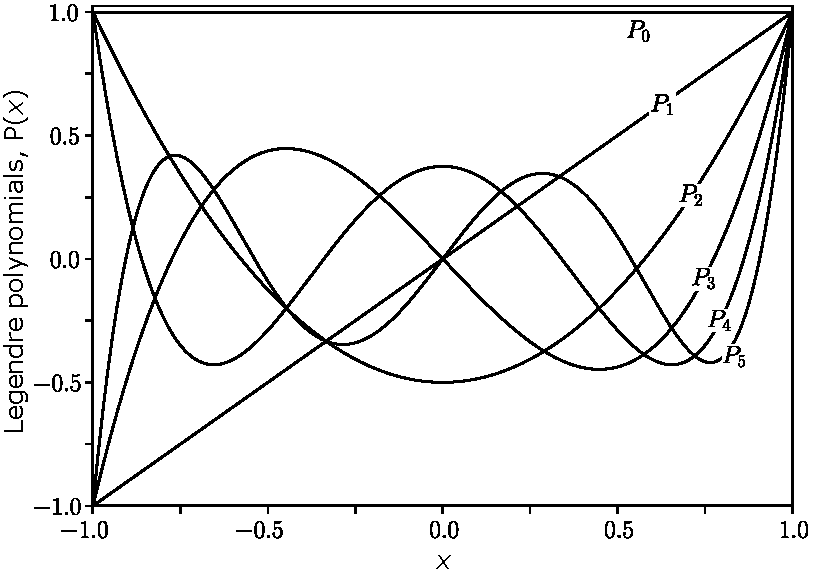
\includegraphics[width = 12cm]{2_legendre.pdf}
    \caption{
        The first six Legendre polynomials ($P_0$ through $P_{5}$) as defined by \autoref{eq:legendre} over the region $[-1, 1]$ for which they are orthogonal.
        Plot adapted from Geek3, \protect\href{https://creativecommons.org/licenses/by-sa/3.0}{CC BY-SA 3.0}, via \protect\href{https://commons.wikimedia.org/wiki/File:Legendrepolynomials6.svg}{Wikimedia Commons} (2023).
    }
    \label{fig:legendre}
\end{figure}

\paragraph{Legendre Polynomials}

Similar to the Chebyshev polynomials, the Legendre polynomials may be defined explicitly as:
\begin{align} \label{eq:legpolyexplicit}
    P_{n}(x) &= \frac{1}{2^{n} n!} \frac{d^{n}}{d x^{n}} (x^{2} - 1)^{n}\,,
\end{align}
or recursively as:
\begin{align}
    P_{0}(x) &= 1 \,,\notag\\
    P_{1}(x) &= x \rlap{\,,\ and} \label{eq:legpoly}\\
    (n+1)P_{n+1}(x) &= (2n+1)xP_n(x) - nP_{n-1}(x) \rlap{\,,\ for $n \geq 1$\,,}\notag
\end{align}
where $P$ is a Legendre polynomial of order $n$.
Legendre polynomials also hold the property of orthogonality.
This means that the inner product of any two differing Legendre polynomials, $P_{i}(x)$ and $P_{j}(x)$, over the range $[-1, 1]$ is zero, as shown by:
\begin{equation} \label{eq:legorth}
    \int_{-1}^{1} P_{i}(x) P_{j}(x) \,dx =
    \begin{cases}
        0,                 & i \neq j \\
        \frac{2}{2 n + 1}, & i = j
    \end{cases}\,,
\end{equation}
where a weight of $1$ is the weighting factor for Legendre polynomials \citep{numerical_recipes, leg}.
A Legendre approximation of an unknown wavelength calibration function is given by:
\begin{align} \label{eq:legendre}
    f(x) &\approx \sum_{n = 0}^{N} a_{n} P_{n}(u) \rlap{\,,\ or}\\
    F(x, y) &\approx \sum_{i = 0}^{N} \sum_{j = 0}^{M} a_{ij} P_{i}(u) P_{j}(v)\,,\label{eq:Legendre2D}
\end{align}
for a one-dimensional wavelength function or a two-dimensional surface function, respectively.
Here $N$ and $M$ are the desired $x$ and $y$ orders, $u$ and $v$ are the same mapping variable as in \autoref{eq:XtoUV}, and $a_{ij}$ are the Legendre polynomial coefficients.

Legendre polynomials benefit from having the orthogonality condition with no weight necessary ($w = 1$) which makes their coefficients computationally easier to compute but increases the error in a Legendre approximation when compared to that of the error in a Chebyshev approximation for functions of the same order, $N$ \citep{leg_cheb_relation}.
% for one-dimensional Legendre and Chebyshev approximations

Regardless of which method of polynomial approximation is chosen, the polynomials are fit by varying the relevant coefficients using the least squares method.
The resultant minimized function may then be used to convert the science frames from an $(x$-pixel$, y$-pixel$)$ coordinate system to a $(\lambda, y$-pixel$)$ coordinate system.


\section{Polarimetry} \label{sec:polarimetry}

% Origin of polarimetry (short history)
Both Huygens and Newton came to the conclusion that light demonstrates transversal properties \citep{Huygens, opticks}, which was later further investigated and coined as `polarization' by Malus \citep{Pol_Malus}.
Malus also investigated the polarization effects of multiple materials including some of which were birefringent, such as optical calcite, which he referred to as Iceland spar after Bartholinus' investigations of the material \citep{Bartholinus}.

% Malus' law gives:
% \begin{equation}
%     I = I_{0} \cos^{2} \theta
%     \label{eq:Malus}
% \end{equation}
% \noindent where $I_{0}$ and $I$ are the Intensity of light before and after polarization, and $\theta$ is the orientation of the polarizer to the direction of propogation of the polarized light.

Fresnel built on Malus' work showing that two beams of light, polarized at a right angle to one another, do not interfere, conclusively proving that light is transversal in nature, opposing the widely accepted longitudinal nature of light due to the prevalent belief in the ether.
He later went on to correctly describe how polarized light is reflected and refracted at the surface of optical dielectric interfaces, without knowledge of the electromagnetic nature of light.
Fresnel's equations for the reflectance and transmittance, $R$ and $T$, are defined as:
\begin{equation} \label{eq:Fresnel}
    \begin{aligned}
        R_{s} &= \left\lvert \frac{Z_{2} \cos{\theta_{i}} - Z_{1} \cos{\theta_{t}}}{Z_{2} \cos{\theta_{i}} + Z_{1} \cos{\theta_{t}}} \right\rvert^{2}\,,\\
        R_{p} &= \left\lvert \frac{Z_{2} \cos{\theta_{t}} - Z_{1} \cos{\theta_{i}}}{Z_{2} \cos{\theta_{t}} + Z_{1} \cos{\theta_{i}}} \right\rvert^{2}\,,\\
        T_{s} &= 1 - R_{s}\,,\ \text{and}\\
        T_{p} &= 1 - R_{p}\,,
    \end{aligned}
\end{equation}
where $s$ and $p$ are the two polarized components of light perpendicular to one another, $Z_{1}$ and $Z_{2}$ are the impedance of the two media, and $\theta_{i}$, $\theta_{t}$, and $\theta_{r}$ are the angles of incidence, transmission, and reflection, respectively \citep{Fresnel}.

Nicol was the first to create a polarizer, aptly named the Nicol prism, where the incident light is split into its two perpendicular polarization components, namely the ordinary and extraordinary beams.
Faraday discovered the phenomenon where the polarization plane of light is rotated when under the influence of a magnetic field, known as the Faraday effect.
Brewster calculated the angle of incidence, $\theta_{B} = \arctan{n_{2} / n_{1}}$, at which incident polarized light is perfectly transmitted through a transparent surface, with refractive indexes of $n_{1}$ and $n_{2}$, while non-polarized incident light is perfectly polarized when reflected and partially polarized when refracted.

Stokes' work created the first consistent description of polarization and gave us the Stokes parameters which describe an operational approach to measuring polarization (discussed further in \autoref{subsec:pol}) \citep{Stokes}.
Hale was the first to apply polarization to astronomical observations, using a Fresnel rhomb and Nicol prism as a quarter-wave plate and polarizer, respectively \citep{Hale_pre,Hale_post}.
Wollaston also created a prism, similarly named the Wollaston prism, which allowed simultaneous observation of the ordinary and extraordinary beams due to the smaller deviation angle \citep{WollPrism}.
Finally, Chandrasekhar's work furthered our understanding of astrophysical polarimetry by explaining the origin of polarization observed in starlight as well as mathematically modeling the polarization of rotating stars, which came to be named Chandrasekhar polarization \citep{chandrasekhar}.

\begin{figure}[t]
    \centering
    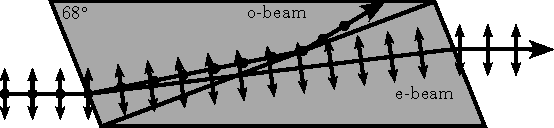
\includegraphics[width=10cm]{2_Nicol_prism.pdf}
    \caption{
        Diagram of a Nicol prism for incident non-polarized light.
        Diagram adapted from Fred the Oyster, \protect\href{https://creativecommons.org/licenses/by-sa/4.0/}{CC BY-SA 4.0}, via \protect\href{https://en.m.wikipedia.org/wiki/File:Nicol_prism.svg}{Wikimedia Commons} (2023).
    }
    \label{fig:Nicol_prism}
\end{figure}

\subsection{Polarization} \label{subsec:pol}

Maxwell's equations for an electromagnetic field propagating through a vacuum are given as:
\begin{equation} \label{eq:Maxwell}
    \begin{gathered}
        \nabla \cdot \matr{E} = 0 \,,\\
        \nabla \cdot \matr{B} = 0 \,,\\
        \nabla \times \matr{E} = - \frac{1}{c} \frac{\partial \matr{B}}{\partial t} \rlap{\,,\ and}\\
        \nabla \times \matr{B} = \frac{1}{c} \frac{\partial \matr{E}}{\partial t}\,,
    \end{gathered}
\end{equation}
where $\matr{E}$ and $\matr{B}$ are the electric and magnetic field vectors, and $c$ is the speed of light.

\enlargethispage{-3\baselineskip}

In a right-handed $(x, y, z)$ coordinate system, a non-trivial solution of an electromagnetic wave following \hyperref[eq:Maxwell]{Maxwell's Equations} propagating along the $z$-axis, towards a hypothetical observer, is described by:
\begin{equation} \label{eq:Maxwell_sol}
    \begin{aligned}
        \matr{E} &= E_{x} \cos(kz - \omega t + \Phi_{x}) \hat{\boldsymbol{x}} +
        E_{y} \cos(kz - \omega t + \Phi_{y}) \hat{\boldsymbol{y}} \rlap{\,,\ and}\\
        \matr{B} &= \frac{1}{c} E_{y} \cos(kz - \omega t + \Phi_{y}) \hat{\boldsymbol{x}} +
        \frac{1}{c} E_{x} \cos(kz - \omega t + \Phi_{x}) \hat{\boldsymbol{y}}\,,
    \end{aligned}
\end{equation}
where $E_{x}$, $E_{y}$, $\Phi_{x}$, and $\Phi_{y}$ are all parameters describing the amplitude and phase of the electric field vector in the $(x, y)$ plane, and with the magnetic field vector proportional and perpendicular to the electric field vector \citep{Griffiths}.

Considering only the electric field component and rewriting \autoref{eq:Maxwell_sol} using complex values allows us to simplify the form of the solution to:
\begin{equation} \label{eq:E_field_vector}
    \matr{E} = \Re(\matr{E}_{0} e^{-i \omega t})\,,
\end{equation}
where we only consider the real part of the equation, and where $\matr{E}_{0}$ is defined as:
\begin{equation} \label{eq:pol_vector}
    \matr{E}_{0} = E_{x} e^{i \Phi_{x}} \hat{\boldsymbol{x}} +
    E_{y} e^{i \Phi_{y}} \hat{\boldsymbol{y}}\,,
\end{equation}
and is referred to as the polarization vector since it neatly contains the parameters responsible for the polarization properties \citep{pol_phys}.

% Polarizing Ellipse
\begin{figure}[t]
    \centering
    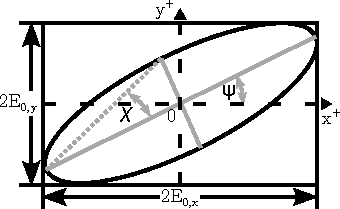
\includegraphics[width=6cm]{2_pol_ellipse.pdf}
    \caption{
        The polarization ellipse for an electric field vector propagating through free space.
        Diagram adapted from Inductiveload, \protect\href{https://creativecommons.org/publicdomain/mark/1.0/}{PDM 1.0}, via \protect\href{https://commons.wikimedia.org/wiki/File:Polarisation_ellipse2.svg}{Wikimedia Commons} (2023).
    }
    \label{fig:pol_ellipse}
\end{figure}

For an electric field vector with oscillations in some combination of the $x$ and $y$ axes, the tip of the vector sweeps out an ellipse, as depicted in \autoref{fig:pol_ellipse}.
This ellipse is referred to as the polarization ellipse and has the form:
\begin{equation} \label{eq:pol_ellipse}
    \left( \frac{\matr{E}_{x}}{\matr{E}_{0, x}}\right)^{2} +
    \left( \frac{\matr{E}_{y}}{\matr{E}_{0, y}}\right)^{2} -
    \frac{2 \matr{E}_{x} \matr{E}_{y}}{\matr{E}_{0, x} \matr{E}_{0, y}} \cos\Phi =
    \sin^{2} \Phi\,,
\end{equation}
where $\Phi = \Phi_{x} - \Phi_{y}$ is the phase difference between the $x$ and $y$ phase parameters.
The degree of polarization for the polarization ellipse is related to the eccentricity of the ellipse and the angle at which it is rotated relates to the polarization angle.
Since $\matr{E}_{0, x}$, $\matr{E}_{0, y}$, $\Phi_{x}$, and $\Phi_{y}$ describe the wave, the polarization ellipse that results from these parameters is fixed as the wave continues to propagate.

\enlargethispage{-4\baselineskip}

Since observations consist of images taken over a desired exposure time, time averaging of \autoref{eq:pol_ellipse} over the exposure time is necessary.
Given the periodical nature and high frequencies of the fields, the time averaging may be found over a single oscillation using:
\begin{equation} \label{eq:pol_t_avg}
    \avg{\matr{E}_{i} \matr{E}_{j}} = \lim_{dt \rightarrow \infty} \frac{1}{T} \int_{0}^{T} \matr{E}_{i} \matr{E}_{j}\,dt\,,\quad \text{for } i, j \in (x, y)\,,
\end{equation}
where $T$ is the total averaging time over the electric field vectors $\matr{E}_{i}$ and $\matr{E}_{j}$ \citep{field_guide}.
Applying the time averaging to \autoref{eq:pol_ellipse} and simplifying results in:
\begin{equation} \label{eq:pol_ellipse_alt}
    (E_{0x}^{2} + E_{0y}^{2})^{2} - (E_{0x}^{2} - E_{0y}^{2})^{2} - (2 E_{x} E_{y} \cos \Phi)^{2} = (2 E_{x} E_{y} \sin \Phi)^{2}\,.
\end{equation}
The expressions inside the parentheses can be found through observation and may also be represented as:
\begin{equation} \label{eq:Stokes_params}
    \matr{S} =
    \begin{pmatrix}
        S_{0} \\
        S_{1} \\
        S_{2} \\
        S_{3}
    \end{pmatrix}
    =
    \begin{pmatrix}
        I \\
        Q \\
        U \\
        V
    \end{pmatrix}
    =
    \begin{pmatrix}
        E_{0x}^{2} + E_{0y}^{2}   \\
        E_{0x}^{2} - E_{0y}^{2}   \\
        2 E_{0x} E_{0y} \cos \Phi \\
        2 E_{0x} E_{0y} \sin \Phi
    \end{pmatrix}\,,
\end{equation}
where $S_{0}$ to $ S_{3}$ are referred to as the Stokes (polarization) parameters.
The parameters describe the: $S_{0}$, total intensity (often normalized to $1$); $S_{1}$, ratio of the \gls{LHP} to \gls{LVP} light; $S_{2}$, ratio of the \gls{L45P} to \gls{L-45P} light; and $S_{3}$, ratio of the \gls{RCP} (clockwise) to \gls{LCP} (counter-clockwise) light.
When the intensity is normalized, the Stokes parameters range from $1$ to $-1$, based on the dominating component of the parameter \citep{Stokes, chandrasekhar}.

% There is, however, a seemingly small, albeit major, shortcoming of the polarization as defined in \autoref{eq:pol_params}; the polarization ellipse as represented by \autoref{fig:pol_ellipse} deals only with a single transverse wave and is incapable of handling a collection of waves which create a wave-packet.
% This is because the waves making up a wave-packet will not share their polarization properties and will temporally vary from one another.
% By taking the time average of the waves in a wave-packet, which happens inherently in the process of observations, this temporal variation may be eliminated.

From \autoref{eq:pol_ellipse_alt} and \ref{eq:Stokes_params}, the polarization parameters are related by:
\begin{equation}
    {I}^{2} = {Q}^{2} + {U}^{2} + {V}^{2}\,,
\end{equation}
for entirely polarized light.
Only beams of completely polarized light could be accounted for before Stokes' work on polarization.
Using the \hyperref[eq:Stokes_params]{Stokes parameters}, we can now account for partially polarized light such that:
\begin{equation}
    I^{2} \geq  Q^{2} + U^{2} + V^{2}\,,
\end{equation}
where $I, Q, U, \text{ and } V$ are the normalized polarization parameters, often symbolized as
\begin{equation} \label{eq:Stokes_norm}
    \bar{Q} = \frac{Q}{I}\,,\quad \bar{U} = \frac{U}{I}\,,\quad \text{and}\quad \bar{V} = \frac{V}{I}\,.
\end{equation}

Similar to the polarization ellipse, the Stokes parameters may be depicted using the Poincar{\'e} sphere in spherical coordinates $(IP, 2 \Psi, 2 \chi)$, such that:
\begin{equation} \label{eq:poincare_coords}
    \begin{aligned}
        I &= S_{0}\,,\\
        P &= \frac{\sqrt{S_{1}^2 + S_{2}^2 + S_{3}^2}}{S_{0}} \rlap{\,,\ for $0 \leq P \leq 1$\,,}\\
        2 \Psi &= \arctan \frac{S_{3}}{\sqrt{S_{1}^{2} + S_{2}^{2}}} \rlap{\,,\ and}\\
        2 \chi &= \arctan \frac{S_{2}}{S_{1}}\,,
    \end{aligned}
\end{equation}
where $I$ denotes the total intensity, $P$ denotes the degree of polarization, or the ratio of polarized to non-polarized light in the wave-packet, $\chi$ denotes the polarization angle, and $\Psi$ denotes the ellipticity angle of the polarization ellipse.

\begin{figure}[t]
    \centering
    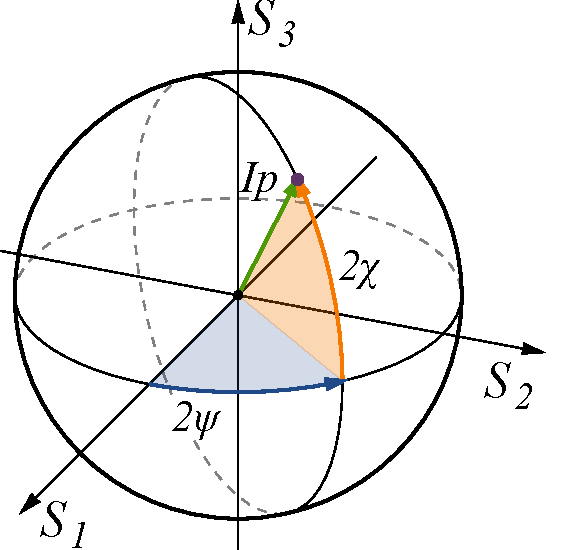
\includegraphics[width=6cm]{2_poincare_sphere.pdf}
    \caption{
        The Poincar{\'e} sphere describing the polarization properties of a wave-packet propagating through free space.
        Diagram adapted from Inductiveload, \protect\href{https://creativecommons.org/publicdomain/mark/1.0/}{PDM 1.0}, via \protect\href{https://commons.wikimedia.org/wiki/File:Poincaré_sphere.svg}{Wikimedia Commons} (2023).
    }
    \label{fig:poincare}
\end{figure}

% Special cases, (1, \pm1, 0, 0), (1, 0, \pm1, 0), (1, 0, 0, \pm1), (1, 0, 0, 0)
% Mueller matrix
% \citep{pol_in_spectra}

% - practically
% Waveplate and polarizer
\subsection{Polarization Measurement} \label{subsec:pol_measure}

Except for polarimetry in the radio-wavelength regime, the polarization of a beam can not be directly measured.
The polarization properties may, however, be recovered from the beam through the manipulation of the four parameters given in \autoref{eq:Maxwell_sol}.
This so-called manipulation is achieved by passing the beam through optical elements which vary the beam for differing amplitudes and phases.
These matrix operations may be represented by their corresponding Mueller matrices.

For ideal components, the resultant beam $\matr{S}^{\prime}$ after passing through an optical element is given by $\matr{S}^{\prime} = \matr{M} \matr{S}$, where $\matr{S}$ is the beam incident on the optical element and $\matr{M}$ represents the $4 \times 4$ Mueller matrix representing the optical element.
Mueller matrices are especially useful when dealing with paths through optical elements as they observe the `train' property \citep{Mueller_train}.
This means that an incoming beam $\matr{S}$ passing, in order, through elements with known Mueller matrices $(\matr{M}_{0}, \dots, \matr{M}_{N})$ results in an outgoing beam $\matr{S}^{\prime}$ such that:
\begin{equation} \label{eq:mueller_train}
    \matr{S}^{\prime} = \matr{M}_{N} \dots \matr{M}_{0} \matr{S}\,.
\end{equation}

Some Mueller Matrices are given below with angles related to those in \autoref{fig:polarimeter}, measured counter-clockwise in a right-handed coordinate system.

\paragraph{General Rotation}
The Mueller matrix for coordinate space rotations about the origin by an angle $\theta$,
\begin{equation} \label{matrix:rotate}
    \matr{R}(\theta) =
    \begin{bmatrix}
        1 & 0              & 0             & 0 \\
        0 & \cos 2 \theta  & \sin 2 \theta & 0 \\
        0 & -\sin 2 \theta & \cos 2 \theta & 0 \\
        0 & 0              & 0             & 1 \\
    \end{bmatrix}\,.
\end{equation}

\begin{figure}[t]
    \centering
    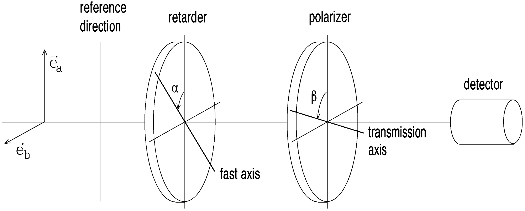
\includegraphics[width=1\textwidth]{2_polarimeter.pdf}
    \caption{
        A diagram of an ideal polarimeter.
        Diagram adapted from \cite{pol_in_spectra}.
    }
    \label{fig:polarimeter}
\end{figure}

\paragraph{General Linear Retardance}
The Mueller matrix for retardance where $\alpha$ is the angle between the incoming vector and fast axis, and $\delta$ is the retardance introduced by the retarder,
\begin{equation} \label{matrix:retarder}
    \matr{W}(\alpha, \delta) =
    \begin{bmatrix}
        1 & 0                                                 & 0                                                 & 0                          \\
        0 & \cos^{2} 2 \alpha + \sin^{2} 2 \alpha \cos \delta & \cos 2 \alpha \sin 2 \alpha  (1 - \cos \delta)    & \sin 2 \alpha \sin \delta  \\
        0 & \cos 2 \alpha \sin 2 \alpha  (1 - \cos \delta)    & \cos^{2} 2 \alpha \cos \delta + \sin^{2} 2 \alpha & -\cos 2 \alpha \sin \delta \\
        0 & -\sin 2 \alpha \sin \delta                        & \cos 2 \alpha \sin \delta                         & \cos \delta                \\
    \end{bmatrix}\rlap{.} 
\end{equation}
The retarder is often referred to by this retardance, e.g., if the retardance is $\delta = \pi$ or $\pi / 2$, the retarder is referred to as a half- or quarter-wave plate, respectively.

\paragraph{General Linear Polarization}
The Mueller matrix for linear polarization where $\beta$ is the angle between the incoming vector and transmission axis,
\begin{equation} \label{matrix:polarizer}
    \matr{P}(\beta) = \frac{1}{2}
    \begin{bmatrix}
        1            & \cos 2 \beta              & \sin 2 \beta              & 0 \\
        \cos 2 \beta & \cos^{2} 2 \beta          & \cos 2 \beta \sin 2 \beta & 0 \\
        \sin 2 \beta & \sin 2 \beta \cos 2 \beta & \sin^{2} 2 \beta          & 0 \\
        0            & 0                         & 0                         & 0 \\
    \end{bmatrix}\,.
\end{equation}

These matrices in combination with \autoref{eq:mueller_train} allow us to describe how the incoming Stokes parameters would change when passing through the various optical elements.
For a setup similar to \autoref{fig:polarimeter}, the detected Stokes parameters can be described by:
\begin{equation} \label{eq:Stokes_intensity}
    \begin{split}
        S^{\prime}(\alpha, \beta, \gamma) \propto \frac{1}{2} \{ I & + [Q \cos2\alpha + U \sin2\alpha] \cos(2\beta - 2\alpha) \\
        & - [Q \sin2\alpha + U \cos2\alpha] \sin(2\beta - 2\alpha) \cos\gamma\\
        & + \,V \sin(2\beta - 2\alpha)\sin\gamma \}\,,
    \end{split}
\end{equation}
where the retandance angle, $\alpha$, polarization angle, $\beta$, for a wave plate with a relative phase difference, $\gamma$, may be varied to acquire a system of equations that can be solved to retrieve the Stokes polarization parameters \citep{waveplate_in_specpol}.

\enlargethispage{-2\baselineskip}

Several or more frames taken under differing configurations may be used to reduce a system of equations to extract all four Stokes polarization parameters, but it is possible to extract the $I$, $Q$ and $U$ polarization parameters using only four frames, or two dual-beam frames, for well-chosen configurations and assuming ideal components.
This ideal configuration varies the retarder angle such that $\Delta\alpha = \pi / 8$ while keeping the polarizer stationary.
More frames for additional retarder angles are advisable and often necessary, however, as they correct for any differences in sensitivity, such as may arise in a polarized flat field and which is further discussed in \autoref{subsubsec:pol_flat} \citep{polarimetry_error}.
From \autoref{eq:Stokes_intensity} we see that the linear retarder element is the driving element of a polarizer as the first three Stokes parameters ($S_{0-2}$, or $I$, $Q$, and $U$) may be found by changing only the angle of retardance, $\alpha$.

\begin{figure}[t]
    \centering
    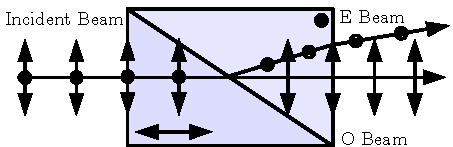
\includegraphics[width=0.5\textwidth]{2_rochon.pdf}
    \caption{
        Diagram of a Rochon prism.
        Included in the diagram are the optical axes of the differing sections of the birefringent material as well as polarizing directions of the incident beam, denoted using the $\leftrightarrow$ and $\odot$ symbols, for the $O$- and $E$-beams, respectively.
        Figure adapted from ChrisHodgesUK, \protect\href{https://creativecommons.org/licenses/by-sa/3.0/}{CC BY-SA 3.0}, via \protect\href{https://commons.wikimedia.org/wiki/File:Rochon_Prism.svg}{Wikimedia Commons} (2023).
    }
    \label{fig:Rochon_prism}
\end{figure}

\paragraph{Wave Plates}
Wave plates, also commonly referred to as retarders, are generally made from optically transparent birefringent crystals.
A wave plate has a fast and slow axis, which are perpendicular to one another and both perpendicular to an incident beam.
Due to the birefringence of the wave plate medium, the phase velocity of the beam polarized parallel to the fast axis, namely the extraordinary beam, slightly increases while that of the beam polarized parallel to the slow axis, namely the ordinary beam, remains unaffected.
This difference in the perpendicular component's phase velocities introduces a relative phase difference between the two beams, $\gamma$, which is given by:
\begin{equation}
    \gamma = \frac{2 \pi \Delta n L}{\lambda_{0}}
\end{equation}
where $\Delta n$ and $L$ refer to the birefringence and thickness of the wave plate medium, respectively, and $\lambda_{0}$ refers to the vacuum wavelength of the beam \citep{Hecht_optics}.

This relative phase difference determines the name of the wave plate, such that the $\gamma = m(\pi/2) $ and $\gamma = m(\pi/4)$ phase differences, for $m \in Z^{+}$, refer to the half- and quarter-wave plates (which are the most common wave plate phases), respectively.
Phase differences with an integer multiple of one another relate to the same phase difference and are referred to as multiple-order wave plates, while wave plates with a phase difference less than an integer multiple are referred to as zero-order wave plates.
Several multiple-order wave plates can be combined by alternatively aligning the fast axis of one to the slow axis of another to create a compound zero-order wave plate \citep{Hale_birefringence}.

\pagebreak

\paragraph{Polarizers} \label{par:polarizer}
Polarizers are typically made from two prisms, of a birefringent material, cemented together with an optically transparent adhesive.
The actual effect of separating the perpendicular polarization components is achieved using varying effects, namely through:
\begin{itemize}
    \item absorption of one of the polarized components, such as in Polaroid polarizing filters,
    \item total internal reflection of a single polarized component, such as in a Nicol prism (\autoref{fig:Nicol_prism}),
    \item Refraction of a single polarized component, such as in a Rochon prism (\autoref{fig:Rochon_prism}), or
    \item Refraction of both polarization components in differing directions, such as in a Wollaston prism (\autoref{fig:Wollaston_prism}).
\end{itemize}

\begin{figure}[t]
    \centering
    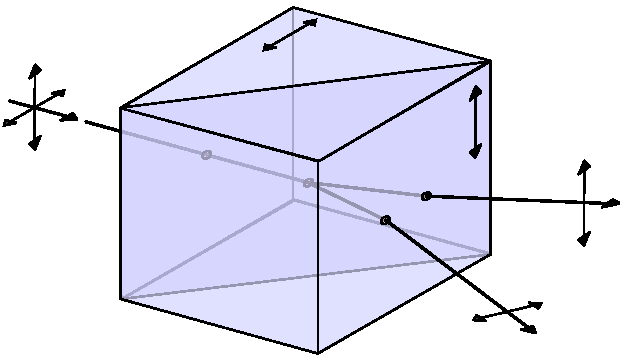
\includegraphics[width=0.5\textwidth]{2_wollaston.pdf}
    \caption{
        Diagram of a Wollaston prism.
        Included in the diagram are the optical axes of the differing sections of the birefringent material as well as polarizing directions of the incident beam, denoted using the $\leftrightarrow$ and $\updownarrow$ symbols, for the $O$- and $E$-beams, respectively.
        Diagram adapted from fgalore, \protect\href{https://creativecommons.org/licenses/by-sa/3.0/}{CC BY-SA 3.0}, via \protect\href{https://commons.wikimedia.org/wiki/File:Wollaston-prism.svg}{Wikimedia Commons} (2023).
    }
    \label{fig:Wollaston_prism}
\end{figure}

\paragraph{Wollaston Prisms} \label{par:wollaston}
The Wollaston prism consists of two right-angle prisms consisting of a birefringent monoaxial material, cemented together with an optically transparent adhesive along their hypotenuses with their optical axes orthogonal, as seen in \autoref{fig:Wollaston_prism}.
The Wollaston prism is a common optical polarizing element in astrophysical polarimetry which separates an incident beam into two linearly polarized $O$- and $E$-beams, orthogonal to one another, and deviated from their common axis equally.
The deviation angle of the polarized beams is determined by both the wedge angle, defined as the angle from the common hypotenuse to that of the outer transmission face of either prism, as well as the material making up the prisms.

Wollaston prisms benefit over simpler elements (such as those listed in the \hyperref[par:polarizer]{polarizer} paragraph) since a single frame allows for the observation of both orthogonal polarization components.
This halves the observational time required to collect enough data to calculate the Stokes parameters, at the cost of an increase in calibration and reduction difficulty \citep{wollaston}.

\subsection{Polarimetric Calibrations} \label{subsec:pol_cal}

The raw science images acquired during polarimetric observations contain a combination of useful science data as well as noise.
Corrections and calibrations related to the detector remain unchanged from those described in \autoref{subsec:calibration}, while those related to correcting for the optical elements relate to corrections for spurious polarization effects.

\subsubsection{Flat Fielding} \label{subsubsec:pol_flat}

Once the \gls{CCD} calibrations have been completed, the polarization intrinsic to the optical elements needs to be accounted for such that the pixel-to-pixel response is made uniform.
Flat-fielding is, once again, used to correct for this.
The flats taken for polarimetry, however, introduce an additional challenge as the targets for conventional flats are polarized, such as twilight and dome flats which are polarized by light scattering in the atmosphere and the reflective surface of the dome, respectively.

If no unpolarized flat images can be taken for flat field calibrations then, when possible due to the polarimeter design, the wave plate may be constantly rotated to act as a depolarizing element; this is effective so long as the wave plate rotation period is much faster than the flat's exposure time.
Alternatively, polarized flats may be taken at the same set of half-wave plate angles used for science observations and averaged together to achieve a similar depolarizing effect.

Observing additional `redundant' exposures for the science and flat images increases the depolarizing effect up to the maximum of $16$ half-wave plate positions, where exposures with a half-wave plate angle differing by $\pi / 4$ from another are considered redundant due to the $O$- and $E$-beams swapping between the related exposures.

Increasing the amount of redundant observations proportionally increases the time needed to observe all the exposures, which in turn introduces time-dependent effects such as fringing or intensity variations of the flat source.
As such, a middle ground must be found for the amount of redundant frames observed \citep{polarimetry_error, pol_optimize}.

\subsubsection{Dual-Beam Extraction and Alignment} \label{subsubsec:pol_oe_extract}

After calibrations for the \gls{CCD} and light path are accounted for, the $O$- and $E$-beams can be extracted and further reduced.
The extraction depends heavily on the layout of the polarimeter but often a simple cropping of the differing sections is enough to separate the two images.

% Image Alignment
After extracting the $O$- and $E$-beams for a specific half-wave plate angle, the images need to be aligned such that the sources present in them overlap.
The Wollaston prism needs to be corrected for as it introduces a beam deviation which differs across both images.
The aligning of the $O$- and $E$-beams is crucial as the comparison of the dual images is what allows for the calculation of the polarization properties.

\subsubsection{Sky Subtraction} \label{subsubsec:pol_sky_subtract}

The polarization introduced by the sky introduces a difference in the intensity of the background sky and needs to be removed as it will influence the polarization results of the target source.
Thankfully, the background polarization is an additive type of noise and may be subtracted out across the frames.
This subtraction is done independently for both beams in a frame and for each frame since the background intensity of all observed polarimetric beams will differ based on the observational parameters.

\section{Spectropolarimetry} \label{sec:spectropolarimetry} % In depth

As the name suggests, spectropolarimetry is the measurement of the polarization of light for a chosen spectral range and provides polarimetric results as a function of wavelength.
As spectropolarimetry is so closely reliant on both spectroscopy and polarimetry, advancements in spectropolarimeters have always been gated by the advancements of spectrometers and polarimeters (as described in \autoref{sec:spectroscopy} and \autoref{sec:polarimetry}).

The most notable historical contributions of spectropolarimetry are those of spectropolarimetric studies instead of instrumental developments.
Spectropolarimetry provides further insights into a materials physical structure, chemical composition, and magnetic field, allowing spectropolarimetry to be useful across multiple disciplines.
In astronomy in particular, spectropolarimetry has been used to study the magnetic field, chemical composition, and underlying structure and emission processes of multiple types of celestial objects \citep[see for example][]{specpol_AGN, specpol_stars, specpol_SN}.

\begin{figure}[t]
    \centering
    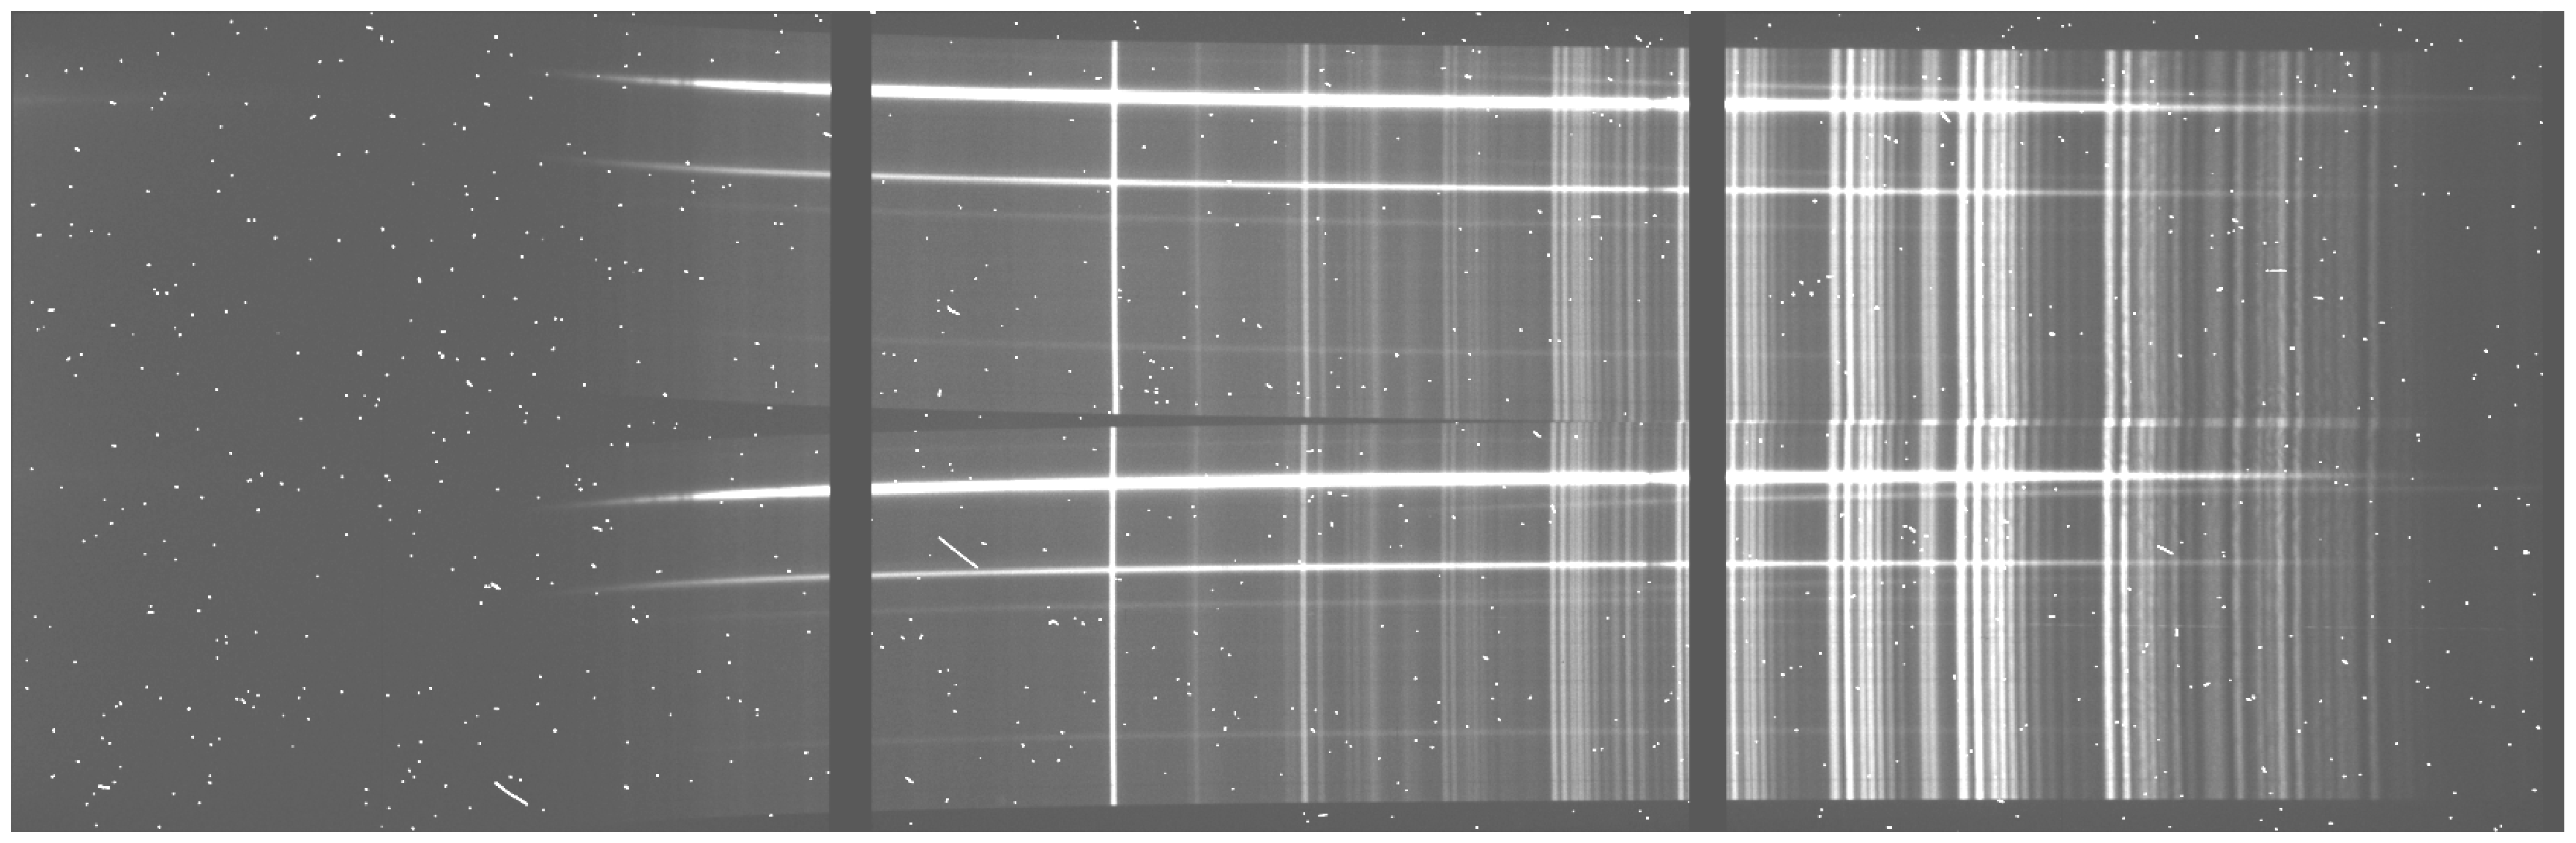
\includegraphics[width=1.0\textwidth]{2_specpol_sci.pdf}
    \caption{A spectropolarimetric target exposure as observed by the \gls{SALT}/\gls{RSS} in spectropolarimetry mode.}
    \label{fig:specpol_exp}
\end{figure}

Along with common points of consideration when developing any instrumentation for observational astronomy, such as resolution and sensitivity, spectropolarimeters need also consider the spectral response of the polarimetric components as well as the polarization response of the spectroscopic components as both are simultaneously in the light-path during observations and have noticeable affects on one another.
Time is another constraint for spectropolarimetry as the incident light is separated both by wavelength and by polarization states.
This division of the incident light results in increased exposure times for both target observations and observations necessary for calibrations.

\autoref{fig:specpol_exp} illustrates a typical science image taken with a spectropolarimeter.
The image contains the $O$- and $E$-beams which are both dispersed into their spectra.
Spectropolarimetric results are acquired from measurements and calibrations of these images alongside any necessary calibration images.

\pagebreak

\subsection{Spectropolarimetric Measurement}

The derived relations given in \autoref{subsec:pol}, such as the \hyperref[eq:Stokes_params]{Stokes parameters}, describe polarization in general and are valid for both polarimetry and spectropolarimetry.
Due to the time averaging of the observed light (\autoref{eq:pol_t_avg}), any minor temporal variation, partial polarization, or monochromatic nature of the spectropolarimetric polarization parameters are accounted for.

For linear spectropolarimetry using a dual-beam polarizing element, an exposure measures the $O$- and $E$-beam wavelength dependent intensities, $f_{O, i}(\lambda)$ and $f_{E, i}(\lambda)$, for a given wave plate angle $\theta_{i}$ at angle $i$.
These intensities thus relate to the wavelength dependent Stokes parameters as:
\begin{equation} \label{eq:specpol_flux_to_Stokes}
    \begin{aligned}
        f_{O, i}(\lambda) &= \frac{1}{2} [I(\lambda) + Q(\lambda)\cos(4\theta_{i}) + U(\lambda)\sin(4\theta_{i})] \rlap{\,,\ and}\\
        f_{E, i}(\lambda) &= \frac{1}{2} [I(\lambda) - Q(\lambda)\cos(4\theta_{i}) - U(\lambda)\sin(4\theta_{i})]\,.
    \end{aligned}
\end{equation}
At least four linear equations are required to solve for three variables in a system of linear equations and thus at least two exposures must be taken to solve for the linear ($I(\lambda)$, $Q(\lambda)$, and $U(\lambda)$) polarization parameters \citep{pol_std, keller_instr}.

The first Stokes parameter, $I(\lambda)$, may be recovered for each dual-beam exposure using
\begin{equation} \label{eq:specpol_I_calc}
    I_{i}(\lambda) = f_{O, i}(\lambda) + f_{E, i}(\lambda)\,.
\end{equation}
By calculating the $I_{i}(\lambda)$ Stokes parameter for each wave plate position $i$, the variation of the target over the course of observation may be corrected for, resulting in the $I(\lambda)$ Stokes parameter.

Next, the $Q(\lambda)$ and $U(\lambda)$ Stokes parameters are found by first defining the normalized difference in relative intensities, $F_{i}(\lambda)$, as:
\begin{equation} \label{eq:specpol_norm_flux}
    F_{i}(\lambda) \equiv \frac{f_{O, i}(\lambda) - f_{E, i}(\lambda)}{f_{O, i}(\lambda) + f_{E, i}(\lambda)}\,,
\end{equation}
which allows \autoref{eq:specpol_flux_to_Stokes} to be written, as
\begin{equation} \label{eq:specpol_F_to_params}
    F_{i}(\lambda) = \bar{Q}(\lambda) \cos(4\theta_{i}) + \bar{U}(\lambda) \sin(4\theta_{i}) = P\cos(4\theta_{i} - 2\chi)\,,
\end{equation}
in terms of the normalized Stokes parameters, or, alternatively, the degree of polarization, $P$, and polarization angle, $\chi$ (as described in \autoref{eq:Stokes_norm} and \ref{eq:poincare_coords}).

The optimal change in wave plate angle is $\Delta\theta_{i} = \pi/8$ as it allows the normalized Stokes polarization parameters to be calculated as:
\begin{equation} \label{eq:specpol_Stokes_sol}
    \begin{aligned}
        \bar{Q}(\lambda) &= \frac{2}{N} \sum_{i = 0}^{N - 1} F_{i}(\lambda) \cos\left(\frac{\pi}{2} i\right) \rlap{\,,\ and}\\
        \bar{U}(\lambda) &= \frac{2}{N} \sum_{i = 0}^{N - 1} F_{i}(\lambda) \sin\left(\frac{\pi}{2} i\right)\,,
    \end{aligned}
\end{equation}
where $N$ is the number of exposures taken, limited such that $N \in [2, 16]$ \citep{polarimetry_error}.

% The desired degree of polarization as well as the polarization angle for linear spectro\-polarimetry is calculated as:
% \begin{equation} \label{eq:specpol_results}
%     \begin{aligned}
%         P    &= \sqrt{\bar{Q}^{2} + \bar{U}^{2}} \\
%         \chi &= \frac{1}{2} \arctan \frac{\bar{U}}{\bar{Q}}
%     \end{aligned}
% \end{equation}
% which is derived from \autoref{eq:poincare_coords} or by solving a system of linear equations of \autoref{eq:specpol_F_to_params} \citep{pol_std,keller_instr}.

\subsection{Spectropolarimetric Calibrations} \label{subsec:specpol_cal}

% The calibrations necessary for the measurement to take place are, as always, seemingly more involved than the calculation of the results themselves.
Just as the elements of a spectropolarimeter are an amalgamation of both a spectrometer and polarimeter, it naturally follows that the calibrations necessary to reduce spectropolarimetric data are a combination of the calibrations needed for spectroscopy and polarimetry, discussed further in \autoref{subsec:calibration} and \autoref{subsec:pol_cal}.
Even though the spectrometer and polarimeter components both have an effect on an incident beam following the light-path through the spectropolarimeter, the calibration procedures for both methods remain mostly independent of one another and as such need not be repeated here.

Spectropolarimetric calibrations are, however, more involved when compared to the same calibrations for either spectroscopy or polarimetry.
Minor deviations in the calibrations across both the spectra and the polarized beam compound, especially when dealing with the wavelength calibration, resulting in poor \glspl{SNR}.
Generally, more exposures over longer timespans are required to acquire enough redundancy and signal for the calculation of the Stokes parameters on top of the time necessary for calibrations to be completed.
It should therefore be noted just how important the calibrations are when dealing with spectropolarimetry.

\section{The Southern African Large Telescope} \label{sec:SALT} % Basics, not in depth

\gls{SALT} is a $10$\,m class optical/near-infrared telescope situated at the \gls{SAAO} field station near Sutherland, South Africa \citep{SALT_optical_design}.
The operational design was based on the \gls{HET} situated at McDonald Observatory, Texas, which limits the pointing of the telescope's primary mirror to a fixed elevation ($37$\degree\ from zenith in the case of \gls{SALT}) while still allowing for full azimuthal rotation \citep{HET}.
Both \gls{SALT} and \gls{HET} utilize a spherical primary mirror which is stationary during observations and a tracker housing most of the instrumentation that tracks the primary mirrors spherically shaped focal path.
\autoref{fig:SALT_telescope} depicts \glspl{SALT} tracker (top left), supporting structure, and primary mirror (bottom right).

\begin{figure}[t]
    \centering
    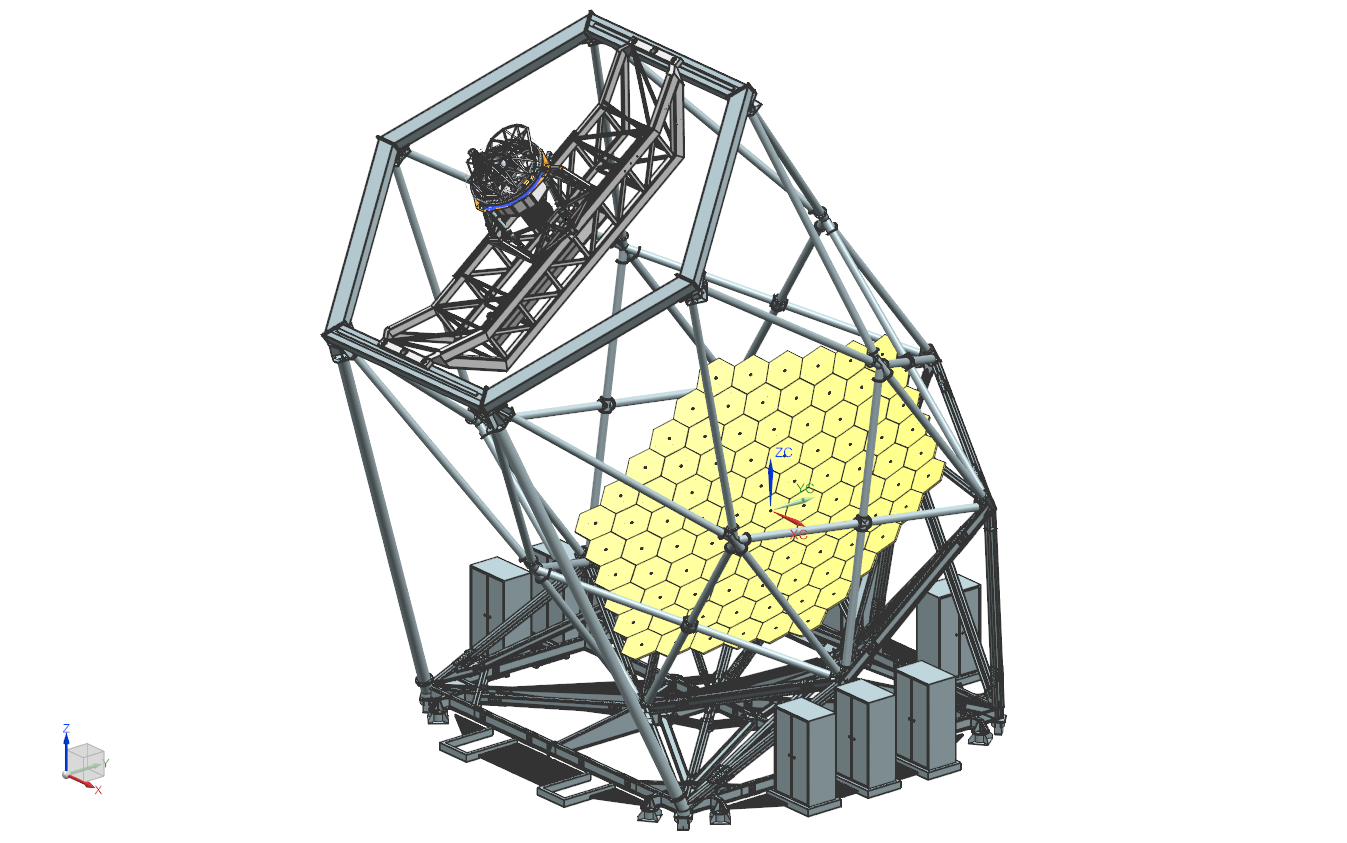
\includegraphics[width=1.0\textwidth]{2_SALT_telescope.png}
    \caption{
        The tracker, supporting structure, and primary mirror of \gls{SALT}.
        Figure adapted from the \gls{SALT} call for proposals \citep{SALT_CFP}.
    }
    \label{fig:SALT_telescope}
\end{figure}

\subsection{The Primary Mirror}

The primary mirror is composed of $91$ individual $1$\,m hexagonal mirrors which together form an $11$\,m segmented spherical mirror.
Each mirror segment can be adjusted by actuators allowing the individual mirrors to approximate a single monolithic spherical mirror.
The fixed elevation means that \glspl{SALT} primary mirror has a fixed gravity vector allowing for a lighter, cost-effective supporting structure when compared to those of a more traditional altitude-azimuthal mount but with the trade-off that the control mechanism and tracking have increased complexity \citep{SALT_design}.

\subsection{Tracker and Tracking}

During observations the primary mirror is stationary and the tracker tracks celestial objects across the sky by moving along the primary focus.
The tracker is capable of $6$ degrees of freedom with an accuracy of $\sim 5$\,$\mu$m and is capable of tracking $\pm 6$\degree\ from the optimal central track position.
As the tracker moves along the track the effective collecting area varies and thus \gls{SALT} has a varying effective diameter of $\sim 7$ -- $9$\,m when the tracker is furthest and closest to the optimal central position, respectively.

Targets are observable within the visibility annulus, as shown in \autoref{fig:SALT_visibility}, between declinations of $10.5$\degree\ and $-75.3$\degree.
It is important to note that because of \glspl{SALT} design, the track length of a source is not the same as the visibility window.

\begin{figure}[t]
    \centering
    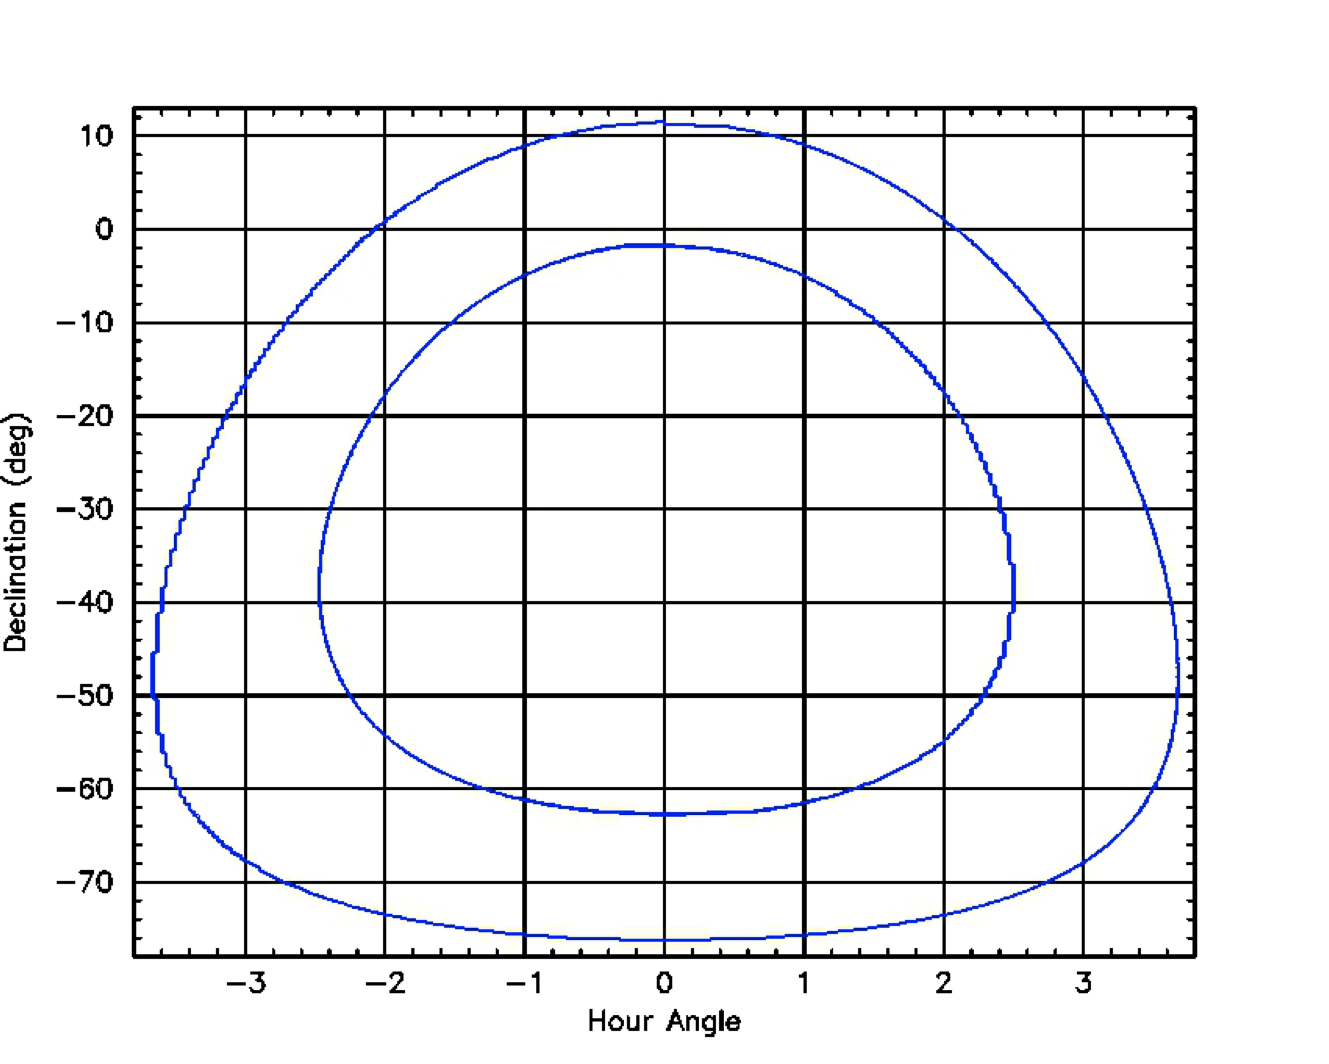
\includegraphics[width = 1.0 \textwidth]{2_SALT_visibility.png}
    \caption{
        The visibility annulus of objects observable by \gls{SALT}.
        Note that the observation windows and observation durations vary based on an object's declination, and that some objects can potentially be observed twice per night, when rising and setting.
        Figure adapted from the \gls{SALT} call for proposals \citep{SALT_CFP}.
    }
    \label{fig:SALT_visibility}
\end{figure}

% Mention Center of Curvature Alignment System? : https://en.wikipedia.org/wiki/Shack%E2%80%93Hartmann_wavefront_sensor

The tracker is equipped with a \gls{SAC} \citep{SALT_SAC}, and an \gls{ADComp} \citep{SALT_ADC}, which corrects for the spherical aberration caused by the geometry of the primary mirror and allows access to wavelengths as short as $3200$\,\AA.
These return a corrected flat focal plane with an $8$\arcmin diameter field of view at prime focus on to the science instruments, with a $1$\arcmin annulus around it used by the tracker in a closed-loop guidance system.
The tracker also houses the calibration system which contains the \gls{Ar}, \gls{CuAr}, \gls{HgAr}, \gls{NeAr}, \gls{ThAr}, and \gls{Xe} wavelength calibration lamps \citep{SALT_cal_sys}.

\subsection[SALT Instrumentation]{\gls{SALT} Instrumentation} \label{subsec:SALT_instr}

\begin{figure}[t]
    \centering
    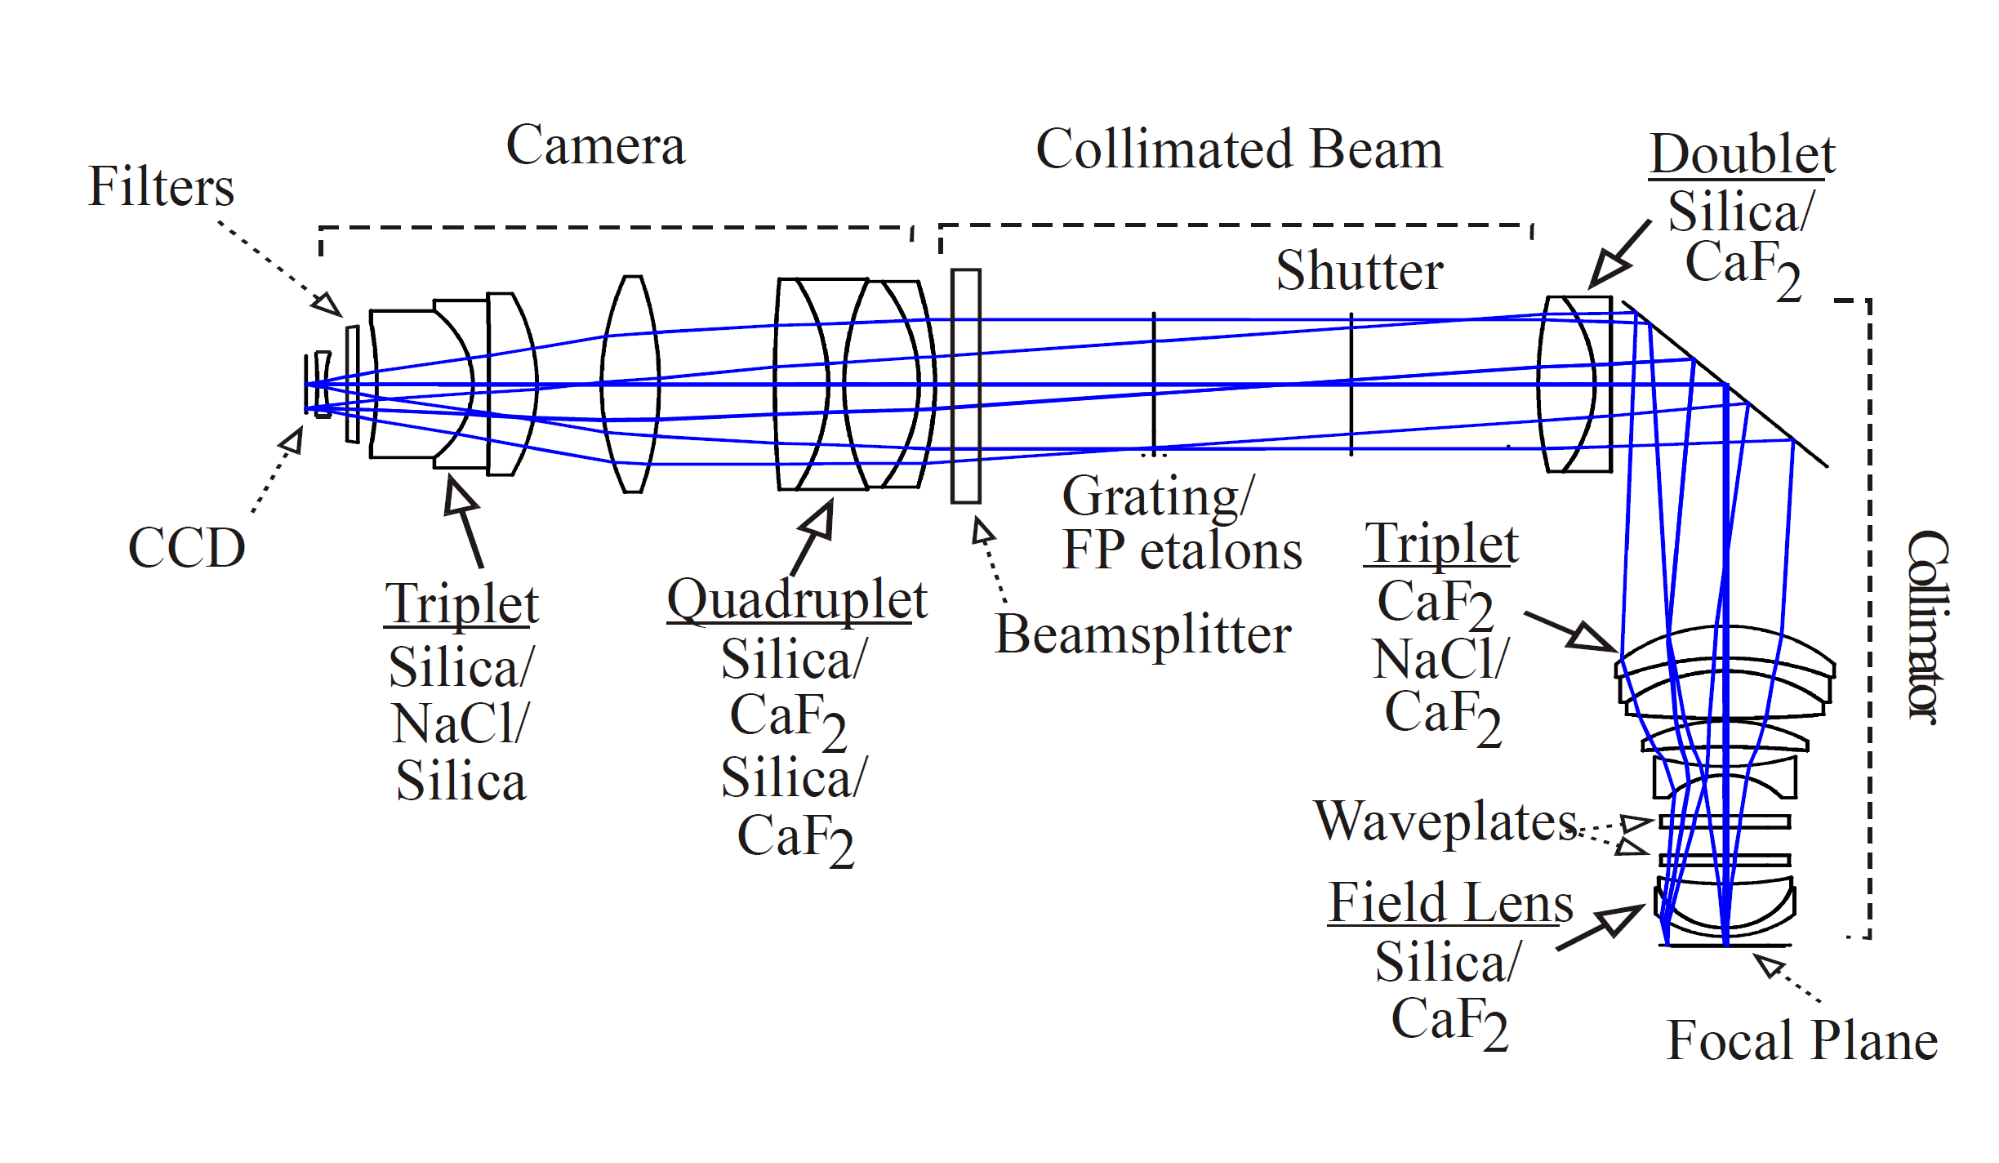
\includegraphics[width = 1.0\textwidth]{2_RSS_optical_path.png}
    \caption{
        The optical path of the \gls{SALT}/\gls{RSS}.
        Figure adapted from the \gls{SALT} call for proposals \citep{SALT_CFP}.
    }
    \label{fig:RSS_layout}
\end{figure}

\Gls{SALT} is equipped with the \gls{SALTICAM} and the \gls{RSS} science instruments onboard the tracker, and the \gls{HRS} and \gls{NIRWALS} science instruments which are fibre-fed from the tracker to their own climate controlled rooms.
The \gls{RSS} is currently the only instrument used for spectropolarimetry.

\subsubsection{\gls{NIRWALS}}

\Gls{NIRWALS} is currently being commissioned and will have a wavelength coverage of $8000$ -- $17000$\,\AA, providing medium resolution spectroscopy at $R = 2000$ -- $5000$ over \glsxtrshort{NIR} wavelengths \citep{NIRWALS, SALT_NIRWALS}.
\gls{NIRWALS} is fibre-fed from its integral field unit and separate sky bundle, consisting of $212$ and $36$ fibers, respectively, housed in the \gls{SALT} fibre instrument feed.
It is ideally suited for studies of nearby galaxies.

\subsubsection{\gls{HRS}}

The \gls{HRS} echelle spectrograph was designed for high resolution spectroscopy at $R = 37000$ -- $67000$ covering a wavelength range of $3700$ -- $8900$\,\AA\ \citep{HRS, HRS_init, SALT_HRS} and consists of a dichroic beam splitter and two \gls{VPH} gratings \citep{SALT_hires}.
This instrument is capable of stellar atmospheric and radial velocity analysis.

\subsubsection{\gls{SALTICAM}}

\Gls{SALTICAM} functions as the acquisition camera and science imager with imaging modes such as full-mode and slot-mode imaging, and supports low exposure times, down to $50$\,ms \citep{SALTICAM}.
This enables photometry of faint objects at short exposures.

\subsubsection{\gls{RSS}} \label{subsubsec:RSS}

The \gls{RSS} functions as the primary spectrograph on \gls{SALT} and can operate in long-slit spectroscopy and spectropolarimetry modes, a narrowband imaging mode, and multi-object and high resolution spectroscopy modes \citep[for an in-depth discussion on operational modes see][]{SALT_operational_modes, SALT_CFP}.

\paragraph{The Detector}
The \gls{RSS} detector consists of a mosaic of three \gls{CCD} chips with a total pixel scale of $0.1267\arcsec$ per unbinned pixel with varying readout times depending on the binning and readout mode.
The mosaicking results in a characteristic double `gap' in the frames and resultant spectra taken with the \gls{RSS}, as seen in \autoref{fig:specpol_exp}.

\paragraph{The Available Gratings}
The \gls{RSS} is equipped with a rotatable magazine of six \gls{VPH} gratings, as listed in \autoref{table:RSS_gratings}.
Observations may be planned using \href{https://astronomers.salt.ac.za/software/}{simulator tools} provided by \gls{SALT} and are performed in the first order only.
The \gls{RSS} has a clear filter, as well as three \gls{UV} (with differing lower filtering ranges) and one blue order blocking filter available, used in conjunction with the various gratings to block out contamination from the second order.

\paragraph{\gls{RSS} Spectropolarimetry} \label{sec:RSS_reductions}

Spectropolarimetry using the \gls{RSS} is currently commissioned for long-slit linear spectro\-polarimetry, $(I, Q, U)$, where observations are taken following the waveplate pattern lists as in \autoref{table:RSS_specpol_patterns}.
Circular, $(I, V)$, and all-Stokes, $(I, Q, U, V)$, spectropolarimetry modes are in commissioning with observations including redundant half-wave plate pairs to be commissioned thereafter.\footnote{Commission status sourced from the latest \href{https://astronomers.salt.ac.za/wp-content/uploads/sites/71/2022/06/3170AM0013_Polarimetry_Observers_Guide_V1.2.pdf}{SALT `Polarimetry Observers Guide' (2024)}.}

\pagebreak

\begin{table}[t]

  \centering

  \caption{Gratings available for use with the \gls{RSS}. Table adapted from the \gls{SALT} call for proposals (2023).}
  \label{table:RSS_gratings}

  \begin{tabular}{lcccc}
    \toprule
    Grating Name &
    \begin{tabular}[c]{@{}c@{}}Wavelength\\Coverage (\angstrom)\end{tabular} &
    \begin{tabular}[c]{@{}c@{}}Usable Angles\\(\degree)\end{tabular} &
    \begin{tabular}[c]{@{}c@{}}Bandpass per tilt\\(\angstrom)\end{tabular} &
    \begin{tabular}[c]{@{}c@{}}Resolving\\Power ($1.25\arcsec$ slit)\end{tabular} \\ \midrule
    PG0300\footnotemark{} & $3700 - 9000$ & $ $ & $3900/4400$ & $250 - 600$ \\
    PG0700\footnotemark[\value{footnote}] & $3200 - 9000$ & $3.0 - 7.5$ & $4000 - 3200$ & $400 - 1200$ \\
    PG0900 & $3200 - 9000$ & $12 - 20$ & $\sim3000$ & $600 - 2000$ \\
    PG1300 & $3900 - 9000$ & $19 - 32$ & $\sim2000$ & $1000 - 3200$ \\
    PG1800 & $4500 - 9000$ & $28.5 - 50$ & $1500 - 1000$ & $2000 - 5500$ \\
    PG2300 & $3800 - 7000$ & $30.5 - 50$ & $1000 - 800$ & $2200 - 5500$ \\
    PG3000 & $3200 - 5400$ & $32 - 50$ & $800 - 600$ & $2200 - 5500$ \\
    \bottomrule
  \end{tabular}

\end{table}
\footnotetext{The PG0300 surface relief grating has been replaced with the PG0700 \gls{VPH} grating as of November 2022 but has been included here as observations using the PG0300 are used in later sections.}


% Tildes (~) are used to indicate spacing for alignment purposes
\begin{table}[t]

    \centering

    \caption{Spectropolarimetry waveplate patterns defined for the \gls{RSS}. The stated angles refer to the angle of the half (\sfrac{1}{2}\,-) and quarter (\sfrac{1}{4}\,-) waveplate's optical axis from the perpendicular of the dispersion axis. Table adapted from the \gls{SALT} call for proposals \citep{SALT_CFP}.}
    \label{table:RSS_specpol_patterns}

    \begin{tabular}{cccccccccc}
        \toprule
        \multicolumn{2}{c}{Linear (\degree)} &
        \multicolumn{2}{c}{Linear-Hi (\degree)} &
        \multicolumn{2}{c}{Circular (\degree)} &
        \multicolumn{2}{c}{Circular-Hi (\degree)} &
        \multicolumn{2}{c}{All Stokes (\degree)} \\
        \sfrac{1}{2} & \sfrac{1}{4} &
        \sfrac{1}{2} & \sfrac{1}{4} &
        \sfrac{1}{2} & \sfrac{1}{4} &
        \sfrac{1}{2} & \sfrac{1}{4} &
        \sfrac{1}{2} & \sfrac{1}{4} \\
        \midrule
        $0$    & - & $0$     & - & $0$ & $45$    & $0$    & $45$    & $0$    & $0$ \\
        $45$   & - & $45$    & - & $0$ & $-45$~~ & $0$    & $-45$~~ & $45$   & $0$ \\
        $22.5$ & - & $22.5$  & - &     &         & $22.5$ & $-45$~~ & $22.5$ & $0$ \\
        $67.5$ & - & $67.5$  & - &     &         & $22.5$ & $45$    & $67.5$ & $0$ \\
               &   & $11.25$ & - &     &         & $45$   & $45$    & $0$    & $45$ \\
               &   & $56.25$ & - &     &         & $45$   & $-45$~~ & $0$    & $-45$~~ \\
               &   & $33.75$ & - &     &         & $67.5$ & $-45$~~ &        & \\
               &   & $78.75$ & - &     &         & $67.5$ & $45$    &        & \\
    \bottomrule
    \end{tabular}

\end{table}

